In this chapter, examples with prompt \verb#-># are written in Scilab environment and examples
with prompt \verb#>># are written in Matlab environment. Examples with prompt \verb#->(>>)#  are available in both environments.\\
In files examples, note that all sequences written between \verb#[#   \verb#]# are comments for users.
%============================
\section{Data representation}
%============================
%====================================
%====================================
\subsection{Individuals representation} \label{individualsRepresentationSection}
%====================================
%====================================
{\sc mixmod} is concerned with data sets where experimental unit
individuals are described with several variables. Individuals are
represented in a standard way a row vector. Then data sets are
represented by a matrix with $n$ rows and $d$ columns, rows representing individuals, and columns representing variables.\\
Let's consider the {\it esteve.dat} individual file, in the directory MIXMOD/DATA, which describes 77 individuals and 7
variables in a \textbf{quantitative situation}

{\scriptsize
\begin{verbatim}
        0.8277   0.3626   0.4243   0.0269   0.0523   0.0000   2.7021
        0.7713   0.4399   0.4586   0.0355   0.0000   0.0015   4.0874
        0.6407   0.4841   0.5302   0.0000   0.2723   0.0000   2.7531
        0.9384   0.2396   0.2436   0.0008   0.0516   0.0000   2.6013

        ...
\end{verbatim}}


Let's consider the {\it b\_conf.dat} individual file, in the directory MIXMOD/DATA, which describes 30 individuals and 8
variables in a \textbf{qualitative situation}

{\scriptsize
 \begin{verbatim}
        1        1        5        1        1        1        1        2
        1        5        1        1        1        4        2        2
        2        2        5        1        1        3        1        1
        1        5        2        1        1        3        2        1

        ...
 \end{verbatim}
}


Notice that the possible values of qualitative data depend on the number of modalities of the variable.
Only integers are authorized and values such as \textit{yes/no} are not allowed.

%==================================
%==================================
\subsection{Weight representation}
%==================================
%==================================
Weights are stored in a vector of real or integer numbers, with $n$ (number of individuals) rows.
Weight is an option of {\sc mixmod} and for example it can represent the repetition of individuals.
Let's consider the weight file {\it geyser.wgt} in the directory MIXMOD/DATA/. It gives the information of all
individuals of {\it geyser.dat} repeated 2 times.\\

%{\noindent {\em Warning CV criterion gives pertinent results only if weights are integer numbers.}}

%=====================================
%=====================================
\subsection{Parameter representation} \label{parameterRepresentationSection}
%=====================================
%=====================================
%Parameters give
%proportions, means and dispersion or proportions, means, subDimensions, parameters Akj,
%parameters Bk and orientation of each mixture
%component.
This representation is used in the case of USER initialization type.\\
\begin{itemize}
 \item Gaussian

$ $

Let's consider the parameter file {\it parameter.init} with 2
clusters, in the directory MIXMOD/DATA/. It gives the values of the unknown mixture model parameters in the quantitative case
{\scriptsize
\begin{verbatim}
        0.367647                [Initial proportion of component 1]
        2.094330   54.750000    [Initial mean of component 1]
        17.280889   0.000000    [Initial variance matrix of component 1]
        0.000000   17.280889


        0.632353                [Initial proportion of component 2]
        4.297930   80.284884    [Initial mean of component 2]
        15.830206   0.000000    [Initial variance matrix of component 2]
        0.000000   15.830206
\end{verbatim}}

\item Multinomial

$ $

Let's consider the parameter file {\it parameter\_qualitatif.init} with 2 clusters in the directory MIXMOD/DATA/.
It gives the values of the unknown mixture model parameters in the qualitative case (with modalities [2;3;4;5])
{\scriptsize
 \begin{verbatim}
        0.2                     [Initial proportion of component 1]
        1  2  3  4              [Initial mean of component 1]
        0.1     0.1             [Initial dispersion array of component 1]
        0.1     0.2     0.1
        0.1     0.1     0.3     0.1
        0.1     0.1     0.1     0.4   0.1


        0.8                     [Initial proportion of component 2]
        2  3  4  5              [Initial mean of component 2]
        0.5     0.5             [Initial dispersion array of component 2]
        0.25    0.25    0.5
        0.1667  0.1667  0.1667  0.5
        0.125   0.125   0.125   0.125   0.5


 \end{verbatim}
}

\item Gaussian High Dimensional

$ $

Let's consider the parameter file {\it parameter\_HD.init} with 2 clusters in the directory
MIXMOD/DATA. It gives the values of the unknown mixture parameters in the gaussian high dimensional (HD)
case
{\scriptsize
\begin{verbatim}
        0.75                                            [Initial proportion of component 1]
        14.842      11.718     32.014    36.81   13.35  [Initial mean of component 1]
        3                                               [Initial subDimension of component 1]
        144.744604  0.214614   0.101925                 [Initial parameter Akj of component 1]
        0.063887                                        [Initial parameter Bk of component 1]
       -0.262423    0.355093   0.004478                 [Initial parameter Bk oforientation array of component 1]
       -0.170051   -0.888586  -0.207320
       -0.601104    0.057918   0.532327
       -0.687179   -0.071419  -0.105660
       -0.262061    0.275444  -0.813918


        0.25                                            [Initial proportion of component 2]
        13.27       12.138     28.102    32.624  11.816 [Initial mean of component 2]
        3                                               [Initial subDimension of component 2]
        99.333875   0.155693   0.138530                 [Initial parameter Akj of component 2]
        0.049261                                        [Initial parameter Bk of component 2]
       -0.259855    0.127732  -0.473221                 [Initial parameter Bk oforientation array of component 2]
       -0.239538    0.555917   0.750006
       -0.587639   -0.078075  -0.049268
       -0.675526    0.144512  -0.205855
       -0.271003   -0.804774   0.410791
\end{verbatim}
}


\end{itemize}






%==============================================
%==============================================
\subsection{Partition representation} \label{partitionRepresentationSection}
%==============================================
%==============================================
A partition gives a classification of the individuals they are affected to a mixture component.\\
It is a matrix (of 0 and 1)
with $n$ rows and $k$ columns, each row corresponding to an individual and each column indicating the group
membership ($0$ if the individual does not belong to the group associated to this column
and $1$ otherwise).\\
Some individuals can have no group assignment they are represented by a
row of $0$.\\
Let's consider the full partition file {\it geyser3clusters.part} in the directory MIXMOD/DATA/. This file gives a
full classification of {\it geyser.dat} for 3 mixture components.

This representation is used in the case of USER\_PARTITION initialization type and/or with known partition.
{\scriptsize
\begin{verbatim}
        0   1   0    [individual 1 in component 2]
        0   0   1    [individual 2 in component 3]
        0   1   0    [individual 3 in component 2]
        0   0   1    [individual 4 in component 3]
        1   0   0    [individual 5 in component 1]

        ...

        0   1   0    [individual 268 in component 2]
        0   0   1    [individual 269 in component 3]
        1   0   0    [individual 270 in component 1]
        0   0   1    [individual 271 in component 3]
        1   0   0    [individual 272 in component 1]
\end{verbatim}}
%{\noindent Let's consider the partial partition file {\it iris.partial.part}, in the directory
%MIXMOD/DATA/, with 3 clusters.}
%{\scriptsize
%\begin{verbatim}
%        1  0  0    [individual 3 in component 1]
%
%        ...
%
%        0  1  0    [individual 60 in component 2]
%
%        ...
%
%        0  0  1    [individual 115 in component 3]
%
%        ...
%
%        0  0  0    [individual 149: unknown partition]
%        0  0  0    [individual 150: unknown partition]
%\end{verbatim}}




%===============================
 \section{{\sc MIXMOD} inputs}
%==============================
This section is aimed to define all the inputs available in {\sc mixmod}
independently of how {\sc mixmod} is used (scilab, matlab, or in command line).





\subsection{{\sc mixmod} required inputs}
\label{input_option}

{\sc mixmod} function needs two required inputs
\begin{itemize}
 \item[1.] {\it data} a matrix $[n,d]$ of individuals ($n$ number of samples, $d$ number of variables),
 \item[2.] {\it nbCluster} a vector of integers representing the number of clusters
                             (several clusters can be in competition),
 \item[-] qualitative case

{\it tabModality} a vector representing the modalities on each variable.

% \item gaussian HD  case

%{\it subDimension} a vector of integers or
%                an integer, representing the intrinsic sub-dimension for each class.
\end{itemize}



Optional inputs can be added to the required ones to precise the execution of {\sc mixmod}.

\subsection{{\sc mixmod} optional inputs}
 \paragraph{Criterion} This option permits to select the criterion giving the best configuration
                         of an execution (model, number of cluster and strategy)
    \begin{itemize}
     \item BIC Bayesian Information Criterion (cf. Section 4.3.1 of Statistical Documentation) ;
     \item ICL Integrated Completed Likelihood (cf. Section 4.3.2 of Statistical Documentation) ;
     \item NEC Entropy Criterion (cf. Section 4.3.3 of Statistical Documentation) ;
     \item CV Cross-Validation (cf. Section 4.3.4 of Statistical Documentation) ;
     \item DCV Double Cross-Validation (cf. Section 4.3.5 of Statistical Documentation).
    \end{itemize}


   {\it Default value is 'BIC'}.

 \paragraph{Model}
Specifying a model different of the default one is possible when informations on the data are known
(for example there is the same number of individuals in each class).\\
{\it Default value is 'Binary\_pk\_Ekjh' for qualitative data (see Table \ref{10models})
or 'Gaussian\_pk\_Lk\_C' for quantitative data (see Table \ref{28models} and Table \ref{16models})}.

\noindent {With gaussian HD models, you have to give subDimensionFree and/or subDimensionEqual parameters.}


\begin{table}[!h]
\caption{The 28 Gaussian Models (Covariance Structure).}
{\small
\label{28models}
\begin{center}
\begin{tabular}{|l|l|}
\hline
Model  & Categories \\
\hline
Gaussian$\_p\_L\_I$               & Spherical \\
Gaussian$\_p\_L_k\_I$             &  \\
\hline
Gaussian$\_p\_L\_B$               & Diagonal \\
Gaussian$\_p\_L_k\_B$             & \\
Gaussian$\_p\_L\_B_k$             & \\
Gaussian$\_p\_L_k\_B_k$           & \\
\hline
Gaussian$\_p\_L\_C$               & General \\
Gaussian$\_p\_L_k\_C$             & \\
Gaussian$\_p\_L\_D\_A_k\_D$       & \\
Gaussian$\_p\_L_k\_D\_A_k\_D$     & \\
Gaussian$\_p\_L\_D_k\_A\_D_k$     & \\
Gaussian$\_p\_L_k\_D_k\_A\_D_k$   & \\
Gaussian$\_p\_L\_C_k$             &\\
Gaussian$\_p\_L_k\_C_k$           & \\
\hline
Gaussian$\_p_k\_L\_I$             & Spherical \\
Gaussian$\_p_k\_L_k\_I$           & \\
\hline
Gaussian$\_p_k\_L\_B$             & Diagonal \\
Gaussian$\_p_k\_L_k\_B$           & \\
Gaussian$\_p_k\_L\_B_k$           & \\
Gaussian$\_p_k\_L_k\_B_k$         & \\
\hline
Gaussian$\_p_k\_L\_C$             & General \\
Gaussian$\_p_k\_L_k\_C$           & \\
Gaussian$\_p_k\_L\_D\_A_k\_D$     & \\
Gaussian$\_p_k\_L_k\_D\_A_k\_D$   & \\
Gaussian$\_p_k\_L\_D_k\_A\_D_k$   & \\
Gaussian$\_p_k\_L_k\_D_k\_A\_D_k$ & \\
Gaussian$\_p_k\_L\_C_k$           & \\
Gaussian$\_p_k\_L_k\_C_k$         & \\
\hline
\end{tabular}
\end{center}}
\end{table}








\begin{table}[!h]
\caption{The 10 Binary Models.}
{\small
\label{10models}
\begin{center}
\begin{tabular}{|l|}
\hline
Model \\
\hline
Binary$\_p\_E$ \\
Binary$\_p\_E_j$ \\
Binary$\_p\_E_k$ \\
Binary$\_p\_E_{kj}$ \\
Binary$\_p\_E_{kjh}$  \\
Binary$\_pk\_E$ \\
Binary$\_pk\_E_j$  \\
Binary$\_pk\_E_k$\\
Binary$\_pk\_E_{kj}$ \\
Binary$\_pk\_E_{kjh}$\\
\hline
\end{tabular}
\end{center}}
\end{table}






\begin{table}[!h]
\caption{The 16 High Dimensional (HD) Models.}
{\small
\label{16models}
\begin{center}
\begin{tabular}{|l|}
\hline
Model \\
\hline
Gaussian\_HD$\_p\_A_{kj}\_B_k\_Q_k\_D_k$ \\
Gaussian\_HD$\_p\_A_{k}\_B_k\_Q_k\_D_k$ \\
Gaussian\_HD$\_p\_A_{kj}\_B_k\_Q_k\_D$ \\
Gaussian\_HD$\_p\_A_{kj}\_B\_Q_k\_D$ \\
Gaussian\_HD$\_p\_A_{k}\_B_k\_Q_k\_D$ \\
Gaussian\_HD$\_p\_A_{k}\_B\_Q_k\_D$ \\
Gaussian\_HD$\_p\_A_{j}\_B_k\_Q_k\_D$ \\
Gaussian\_HD$\_p\_A_{j}\_B\_Q_k\_D$ \\
Gaussian\_HD$\_p_k\_A_{kj}\_B_k\_Q_k\_D_k$ \\
Gaussian\_HD$\_p_k\_A_{k}\_B_k\_Q_k\_D_k$ \\
Gaussian\_HD$\_p_k\_A_{kj}\_B_k\_Q_k\_D$ \\
Gaussian\_HD$\_p_k\_A_{kj}\_B\_Q_k\_D$ \\
Gaussian\_HD$\_p_k\_A_{k}\_B_k\_Q_k\_D$ \\
Gaussian\_HD$\_p_k\_A_{k}\_B\_Q_k\_D$ \\
Gaussian\_HD$\_p_k\_A_{j}\_B_k\_Q_k\_D$ \\
Gaussian\_HD$\_p_k\_A_{j}\_B\_Q_k\_D$ \\
\hline
\end{tabular}
\end{center}}
\end{table}




\paragraph{Weight}
This option is to be used when weight is associated to the data.\\
{\it Default value is 1.}

\paragraph{Partition}
This option is to be used when a partition of the data is already known. \\
{\it Default value is no knownPartition.}


\paragraph{Strategy}
This option permits to define different ways to execute the algorithms available in {\sc mixmod}
(cf. section 3 of Statistical Documentation) .\\

\begin{itemize}
 \item[1.] {\bf initialization} defining the initialization of the strategy.
           There are different ways to initialize an algorithm
           \begin{itemize}
            \item RANDOM Initialization from a random position is a standard way to
initialize an algorithm. This random initial position is obtained by
choosing at random centers in the data set. This simple strategy is
repeated $5$ times (the user can choose the number of times) from
different random positions and the position that maximises the
likelihood is selected.
             \item USER\_PARTITION This option initializes the strategy from a
specified classification (full or partial) of the observations.
This option provides the possibility to use {\sc mixmod} for
Discriminant Analysis and in this case, partition must be full.
             \item USER This option starts the strategy with specified initial values
of the unknown mixture model parameters, i.e. the mixing
proportions and the parameters of the distribution.
             \item SMALL\_EM A maximum of $50$ iterations of the EM algorithm according to the process $n_i$ numbers of iterations
of EM are done (with random initialization) until the SMALL\_EM stop criterion value has been reached
 (cf. Statistical Documentation Equation (14)). This action is repeated until the sum of $n_i$
reaches $50$ iterations (or if in one action $50$ iterations are reached before the stop criterion value).\\
It appears that repeating runs of EM is generally profitable since using a single run
of EM can often lead to suboptimal solutions.
             \item CEM\_INIT  $10$ repetitions of $50$ iterations of the CEM algorithm are done.
One advantage of initializing an algorithm with CEM lies in the fact
that CEM converges generally in a small number of iterations. Thus,
without consuming a large amount of CPU times, several runs of CEM are
performed. Then EM is run with the best solution among the $10$ repetitions.
             \item SEM\_MAX  A run of $500$ iterations of SEM. The idea is that an SEM sequence is
expected to enter rapidly in the neighbourhood of the global maximum
of the likelihood function.
             \item[] {\it Default value is RANDOM.}
           \end{itemize}
 \item[2.] {\bf algorithm} defining the algorithms used in the strategy, the stopping rule and when to stop.
            \begin{itemize}
             \item[a.] Algorithms
                \begin{itemize}
                 \item EM Expectation Maximisation (cf. Section 3.1 of Statistical Documentation),
                 \item CEM Classification EM (cf. Section 3.3 of Statistical Documentation),
                 \item SEM Stochastic EM (cf. Section 3.2 of Statistical Documentation),
                 \item MAP Maximum a Posteriori,
                 \item M Only M step.
                \end{itemize}
             \item[b.] Stopping rules for the algorithm
                \begin{itemize}
                 \item NBITERATION Sets the maximum number of iterations,
                 \item EPSILON Sets relative increase of the log-likelihood criterion.
                 \item NBITERATION$\_$EPSILON Sets the maximum number of iterations and the epsilon value.
                \end{itemize}
               \item[] {\it Default values are 200 NBITERATION of EM with an EPSILON value of 10-4.}
            \end{itemize}
\end{itemize}


{\scriptsize
\begin{table}[h]

\label{optionTable}
\begin{center}
\begin{tabular}{|l|l|l|l|l|}
\hline
Criterion   & Initialization     & Algorithms        & Stopping rules & Models Quantitatif/ Qualitatif\\
\hline

{\bf BIC}         & {\bf RANDOM}             & {\bf EM}                & {\bf NBITERATION\_EPSILON} &{\bf  'Gaussian\_pk\_Lk\_Ck'/ 'Binary\_pk\_Ekjh'}  \\
\hline
CV          & USER               & CEM               & EPSILON & \\
\hline
ICL         & USER\_PARTITION    & SEM               & NBITERATION & \\
\hline
NEC         & SMALL\_EM          & MAP               &  & \\
\hline
DCV         & CEM\_INIT          & M                  & &  \\
\hline
            & SEM\_MAX           &                   & &  \\
\hline
            &                    &                   &  & \\
\hline
\end{tabular}
\end{center}
\caption{{\sc mixmod} options bold strings represent default values. .}
\end{table}}


{\noindent Warning 1 with HD models, only init USER\_PARTITION + M and init USER + MAP
                      (the two steps of Discriminant Analysis)
                        are available.}


{\noindent Warning 2 with CEM algorithm, EPSILON = 0 is allowed.}

{\noindent Warning 3 with SEM algorithm, only NBITERATION is allowed.}


%===============================================
\section{{\sc mixmod} Graphical User Interfaces (GUI)}
%===============================================
This section describes the procedure to use {\sc mixmod} graphical user's interfaces. This procedure is roughly
speaking the same for Scilab and Matlab environments.
The two functions {\em mixmodGraph.sci} (Scilab) and {\em
mixmodGraph.m} (Matlab) are available, in the directory MIXMOD/, to launch {\sc mixmod} graphical
user's interface in Scilab (or Matlab) environment.\\
%After executing {\em initMixmod.sci} Scilab function, or adding {\sc mixmod} path to Matlab path,
%{\sc mixmod} interface can be launched using the following command\\

{\noindent Remark With Scilab, you have to execute {\em initMixmod.sci} and
with Matlab, you have to add {\sc MIXMOD} and {\sc MIXMOD/UTIL/MATLAB} directories to Matlab path before
using {\em mixmodGraph.sci} or {\em mixmodGraph.m}}.

%\begin{tabular}{c|c}
%\begin{minipage}[c]{0.30\columnwidth}%
{\scriptsize
\begin{verbatim}
    -> (>>) mixmodGraph;
\end{verbatim}}
%\end{minipage}%
%&
%\begin{minipage}[c]{0.70\columnwidth}%
%{\scriptsize
%\begin{verbatim}
%    >> mixmodGraph;
%\end{verbatim}}
%\end{minipage}%
%\end{tabular}\\

\noindent{Once {\sc mixmod} is launched, the {\em Main Menu} window appears. It contains
the four following choices}
\begin{itemize}
  \item {\em Discriminant Analysis}, to start discriminant analysis,
  \item {\em Cluster Analysis} (or density estimation), to start cluster analysis,
  \item {\em Demos}, to start demonstration session,
  \item {\em Settings} (only for Scilab), to change the display mode,
  \item {\em Help}, provides further information on {\sc mixmod} software.
\end{itemize}

%-----------------------
%-----------------------
\subsection{Demo menu}
%-----------------------
%-----------------------
We propose to begin by a demonstration session. A first contact
with {\sc mixmod} can be made by clicking on {\em Demos} in {\em Main Menu} and,
selecting a data set example, for instance Birds.% and Old Faithfull Geyser.

%---------------------------------------------------------------
\subsubsection{Example with Birds data set}
%---------------------------------------------------------------
\begin{figure}[!hb]
  \centering
  \includegraphics[width=5.5cm, height=4.5cm]{birds.eps}
  \caption{Birds demonstration: multinomial distribution with three components (general model $[Binary\_{p_k}\_{E_{kjh}}]$ see Table \ref{10models}).}
\end{figure}

%\newpage

%-----------------------------------------------------------------------
%\subsubsection{Example with Old Faithfull Geyser data set}
%See \ref{geyserFig1}.
%-----------------------------------------------------------------------
\begin{figure}[!h]
  \centering
  \includegraphics[width=5.5cm, height=4.5cm]{geyser1.eps}
  \caption{Old Faithful Geyser demonstration: Gaussian mixture model with two components (general model $[p_k\lambda_kC]$ see Table \ref{28models}).}
  \label{geyserFig1}
\end{figure}

%--------------------------------
%--------------------------------
\subsection{Cluster analysis}
%--------------------------------
%--------------------------------

%-------------------------------------------
\subsubsection{Getting started with the GUI}
%-------------------------------------------

%This section describes the whole procedure, including
%\begin{itemize}
%  \item data file selection,
%  \item problem dimension entry,
%  \item number(s) of clusters entry.
%\end{itemize}

By clicking on {\em Cluster Analysis} in {\em Main Menu}, three windows appear
successively to define required inputs for the analysis
\begin{itemize}
  \item a window to enter the problem dimension (number of variables), and the array of modalities in
        qualitative case,

  \item an explorer window to select a data file (.dat file or others),

  \item a window to enter the number of clusters. One or several values can be entered. In this last case, {\sc
  mixmod} returns the number of components giving the best results according to some chosen options.
\end{itemize}


Then cluster analysis can be run immediately by clicking
on {\em Start Cluster Analysis} in the {\em Cluster
Analysis Menu} or options can be chosen (see Section \ref{input_option}).\\
%\begin{figure}[!h]

After running the program, a selection of outputs to be
displayed is proposed in the {\em Output Menu}
\begin{itemize}
 \item {\em View Diagnostics } numerical outputs visualisation mode for
                                 parameters, model(s), criterion(s), classification, probabilities and likelihood ;
 \item {\em  Graphics} graphical outputs visualisation
                         in Figure \ref{geyserFig1}, the screen displays the Old
                         Faithful Geyser results (two components have been used with the
                         Ellipsoidal Gaussian model $[p_k\lambda_kC]$ see Table \ref{28models}).

                          If several criteria have been chosen in cluster analysis options, {\sc mixmod}
                          proposes to choose the criterion for which the output shall be
                          displayed.
 \item {\em Save output variable} to save the output. It can be loaded in Scilab or Matlab
                                    and used with mixmodView function (see Section 3.3.2).\\
    \noindent {Warning the name of the variable to draw is necessary {\bf output}.}
\end{itemize}


\paragraph{Example } consider the {\em output} variable and {\em output.mat} saved in directory MIXMOD/:

\begin{tabular}{c|c}
\begin{minipage}[c]{0.50\columnwidth}%
{\scriptsize
\begin{verbatim}
    -> load('output'); // create the output variable
    -> mixmodView(output);
\end{verbatim}}
\end{minipage}%
&
\begin{minipage}[c]{0.50\columnwidth}%
{\scriptsize
\begin{verbatim}
    >> load('output.mat'); % create the output variable
    >> mixmodView(output);
\end{verbatim}}
\end{minipage}%
\end{tabular}





%{\scriptsize
%\begin{verbatim}
%      -> load('output');      // create the output variable
%      -> mixmodView(output);
%
%      >> load('output.mat'); % create the output variable
%      >> mixmodView(output);
%\end{verbatim}}













\subsubsection{Cluster analysis options} \label{clusterAnalysisOptionsSection}

By clicking on {\em Options} in {\em Cluster Analysis Menu}, the {\em Cluster Analysis Options Menu} appears.
This menu, allows to select cluster analysis options among the following ones (see section \ref{input_option} for
more details)
\begin{itemize}
  \item {\em Model }
   \begin{itemize}
      \item {\em Gaussian Model}     (Gaussian\_pk\_Lk\_C by default),
      \item {\em Qualitative Model} (Binary\_pk\_Ekjh by default),

{\noindent  Remark Gaussian HD models are not available in cluster analysis.}

   \end{itemize}
  \item {\em Criteria} (BIC by default),
  \item {\em Strategy}  (RANDOM initialization and 100 iterations of EM by default),
  \item {\em Weight for data} (1 by default),
 \item {\em Partition} (none by default, if given, it won't change during the execution).
\end{itemize}





%-------------------------------------
%-------------------------------------
\subsection{Discriminant analysis}
%-------------------------------------
%-------------------------------------

%-------------------------------------------
\subsubsection{Getting started with the GUI}
%-------------------------------------------

The user supplies classified observations (training observations) and will
classify optional observations (remaining observations). In practice, the
optional individuals must be given in another
separate file with the same number of columns.

Now suppose that a set of $K$ groups is available and for each
observation, the group from which it arises is known. This group
information is used to design a classification rule that assigns any vector
observation to one of the groups.\\

Discriminant analysis can begin by clicking on {\em Discriminant Analysis} in {\em Main Menu}. Then required
inputs for the analysis on training data must be defined
\begin{itemize}
  \item the problem dimension (number of variables),
  \item the number of clusters of the training observations,
  \item the array of modalities in qualitative case

  \item selecting a training observation file (.dat file),

  \item selecting a {\em full} partition file of training observations (.part file).
\end{itemize}

Discriminant analysis can be run immediately by
clicking on {\em Start Discriminant Analysis} in the {\em Discriminant Analysis Menu} or options can be chosen (see Section \ref{discriminantAnalysisOptions}).

First, {\sc mixmod} runs an M step to obtain a classification rule from the training observations. Moreover, if several models
have been chosen in discriminant analysis options, {\sc mixmod} returns the best model.
After this step, the {\em Information Training Data Menu} appears to select the information on the training
observations to be displayed
\begin{itemize}
	\item{\em Reclassifying information by MAP rule}
		\begin{itemize}
			\item{\em Reclassifying array of samples} displays an array $[K, K]$. Each value $(i,j)$ represents the
percentage of observations in group $i$ classified in the group $j$ after the M step.
			\item {\em List of samples misclassified} displays the list of observations misclassified by
MAP.
		\end{itemize}
	\item{\em CV or DCV information (cf. sections 4.3.4 and 4.3.5 of Statistical documentation)}
		\begin{itemize}
			\item{CV }Reclassifying array of samples by Cross Validation rule and list of samples misclassified.
			\item{DCV }Double Cross Validation rate.
		\end{itemize}
  \item {\em Model Parameter} displays the parameters of the best model.
For gaussian HD models proportions, means, subDimension, parameters Akj, parameters Bk and orientation. For the others
parameters, means and dispersion.
\end{itemize}

By clicking on {\em CONTINUE DISCRIMINANT ANALYSIS}, the user can select a remaining
observations file to continue the analysis.\\

Then {\sc mixmod} runs the second step of discriminant analysis (MAP step with classification rule computed in
the first step). The aim of this step is to assign remaining observations to one of the groups. At the end of the
analysis,
an output can be displayed to see numerical or graphical results.





\subsubsection{Discriminant analysis options} \label{discriminantAnalysisOptions}


By clicking on {\em Options} in {\em
Discriminant Analysis Menu}, the {\em Discriminant Analysis Options Menu} appears.
This menu  allows to select discriminant analysis options
among the following choices
\begin{itemize}
  \item {\em Gaussian Model-Based}  (Gaussian\_pk\_Lk\_C by default) or {\em Model} (Binary\_pk\_Ekjh by default),
{\noindent Remark Gaussian HD models are available, you have to give values for subDimensionFree and/or
subDimensionEqual parameters. The parameter subDimensionEqual can be an integer or an array of integers, the
parameter subDimensionFree can be a vector or an array of vectors.}

  \item {\em Criteria} (CV by default),
  \item {\em Weight for data}.
\end{itemize}

{\it Warning CV criterion gives pertinent results only if weights are integers.}






%------------------------------------------------
%\subsubsection{Discriminant analysis options} \label{discriminantAnalysisOptions}
%------------------------------------------------


%\begin{itemize}
%  \item {\bf{Model option}}\\
%It is the same procedure than model option of cluster
%analysis (see Section \ref{clusterAnalysisOptionsSection}).

%  \item {\bf{Criterion option}}\\
%The {\em Criterion Menu} allows to replace CV criterion by DCV (Double Cross Validation)
%criterion type.

%  \item {\bf{Weight option}}\\
%It is the same procedure than weight option of cluster
%analysis (see Section \ref{clusterAnalysisOptionsSection}). Weight are available for training data only.
%\end{itemize}

%\newpage



%=======================================
\section{{\sc mixmod} toolkit functions}
%=======================================
%==================================
\subsection{{\sc mixmod} function}
%==================================
The functions {\em mixmod.sci} and {\em mixmod.m} (Scilab and Matlab) are
available in the directory MIXMOD/.


{\noindent Remark With Scilab, you have to execute {\em initMixmod.sci} and with Matlab,
you have to add {\sc MIXMOD} and {\sc MIXMOD/UTIL/MATLAB} directories to Matlab path to load
{\sc MIXMOD} toolkit functions.}


%After executing {\em initMixmod.sci} in Scilab, or
%adding {\em mixmod path}
%in Matlab, {\em mixmod} functions can be used alone in a Scilab (or Matlab) program.

The calling sequence is
\begin{itemize}
%{\scriptsize
 \item quantitative case
{\scriptsize
\begin{verbatim}
-> (>>) [output [,outTab, optionalOutput]] = mixmod(data, nbCluster [,'criterion',criterion,
        'model',model,'weight', weight,'strategy',strategy,'partition',partition])

\end{verbatim}
}

%{\scriptsize
% \item quantitative case with HD models
%{\scriptsize
%\begin{verbatim}
%-> (>>) [output [,outTab, optionalOutput]] = mixmod(data, nbCluster [,'criterion',criterion,
%        'model',model,'weight', weight,'strategy',strategy,'partition',partition,
%        'subDimension',subDimension])
%
%\end{verbatim}
%





%{\scriptsize
\item qualitative case
% {\tiny
{\scriptsize
 \begin{verbatim}
 -> (>>) [output [,outTab, optionalOutput]] = mixmod(data, nbCluster, 'tabModality',tabModality
         [,'criterion',criterion,'model',model,'weight',weight,'strategy',strategy,'partition',partition])

 \end{verbatim}
 }
\end{itemize}

%{\it Warning
%In the quantitative case, the option subDimension,
%have to be used in a discriminant analysis situation and with the HD models (cf. Table \ref{16models}).}

\vspace*{0.5cm}

In the following examples, we will either consider quantitative or qualitative data sets. The quantitative data set will
be named {\it geyser} and the qualitative one {\it b\_toby}.\\

The principal differences between qualitative and quantitative treatement is the presence of the variable 'tabModality'
in the qualitative case.
%-------------------------------------------
%-------------------------------------------
\subsubsection{Begining with {\sc mixmod}}

The simplest way (without options) to execute {\sc mixmod} function is
%-------------------------------------------
%-------------------------------------------


\begin{tabular}{c|c}
\begin{minipage}[c]{0.40\columnwidth}%
{\scriptsize
\begin{verbatim}
    -> geyser = read('DATA/geyser.dat',272,2);

    -> b_toby = read('DATA/b_toby.dat',216,4);
\end{verbatim}}
\end{minipage}%
&
\begin{minipage}[c]{0.60\columnwidth}%
{\scriptsize
\begin{verbatim}
    >> geyser = load('DATA/geyser.dat');

    >> b_toby = load('DATA/b_toby.dat');
\end{verbatim}}
\end{minipage}%
\end{tabular}


{\scriptsize
\begin{verbatim}
      -> (>>) nbCluster1 = 2;
      -> (>>) tabModality = [2 ; 2 ; 2 ; 2];
      -> (>>) out1 = mixmod(b_toby, nbCluster1,'tabModality',tabModality);
      -> (>>) nbCluster2 = [2; 3];
      -> (>>) out2 = mixmod(geyser, nbCluster2);

\end{verbatim}}

%\end{enumerate}


%-------------------------------------------
%-------------------------------------------
\subsubsection{Executing {\sc mixmod} with options}


\begin{itemize}

\item criterion a vector of strings (scilab) or a cell array of strings (matlab)


\begin{tabular}{c|c}
\begin{minipage}[c]{0.47\columnwidth}%
{\scriptsize
\begin{verbatim}
    -> criterion = 'BIC';
    -> out = mixmod(geyser, 2, 'criterion',criterion);
    -> criteria = ['BIC'; 'ICL'; 'NEC'];
    -> out = mixmod(geyser, 2 ,'criterion',criteria);

\end{verbatim}}
\end{minipage}%
&
\begin{minipage}[c]{0.58\columnwidth}%
{\scriptsize
\begin{verbatim}
    >> criterion = 'BIC';
    >> out = mixmod(geyser, 2, 'criterion',criterion);
    >> criteria = {'BIC'; 'ICL'; 'NEC'};
    >> out = mixmod(geyser, 2, 'criterion',criteria);

\end{verbatim}}
\end{minipage}%
\end{tabular}



\item models a structure containing three fields name, subDimensionFree, subDimensionEqual defining the caracteristics
      of a model.
%vector of strings (scilab) or cell array of strings (matlab)



\begin{tabular}{c|c}
\begin{minipage}[c]{0.5\columnwidth}%
{\scriptsize
\begin{verbatim}
    -> model = tlist(['model','name','subDimensionFree',
               'subDimensionEqual'],'',[],[]);
    -> model.name = 'Binary_pk_Ekj';
    -> out = mixmod(b_toby,2,'tabModality',tabModality,
                   'model',list(model));

    -> model1 = tlist(['model','name','subDimensionFree',
               'subDimensionEqual'],'Binary_pk_Ek',[],[]);
    -> model2 = tlist(['model','name','subDimensionFree',
               'subDimensionEqual'],'Binary_pk_Ej',[],[]);
    -> model3 = tlist(['model','name','subDimensionFree',
               'subDimensionEqual'],'Binary_pk_E',[],[]);
    -> models = list(model1,model2,model3);
    -> out = mixmod(b_toby,2,'tabModality',tabModality,
                   'model',models);

\end{verbatim}}
\end{minipage}%
&
\begin{minipage}[c]{0.58\columnwidth}%
{\scriptsize
\begin{verbatim}
  >> model = struct('name','','subDimensionFree',
               [],'subDimensionEqual',[]);
  >> model.name = 'Binary_pk_Ekj';
  >> out = mixmod(b_toby, 2, 'tabModality',tabModality,
                   'model',{model});
  >> model1 = struct('name','Binary_pk_Ek','subDimensionFree',
               [],'subDimensionEqual',[]);
  >> model2 = struct('name','Binary_pk_Ej','subDimensionFree',
              [],'subDimensionEqual',[]);
  >> model3 = struct('name','Binary_pk_E','subDimensionFree',
               [],'subDimensionEqual',[]);
  >> models = {model1,model2,model3};
  >> out = mixmod(b_toby, 2, 'tabModality',tabModality,
                    'model',models);

\end{verbatim}}
\end{minipage}%
\end{tabular}



\item weight a vector of real or integer values (scilab and matlab)


\begin{tabular}{c|c}
\begin{minipage}[c]{0.52\columnwidth}%
{\scriptsize
\begin{verbatim}

    -> weight = read('DATA/b_toby.wgt',216,1);
    -> out    = mixmod(b_toby, 2, 'tabModality',tabModality,
                       'weight',weight);

\end{verbatim}}
\end{minipage}%
&
\begin{minipage}[c]{0.52\columnwidth}%
{\scriptsize
\begin{verbatim}
 >> weight = load('DATA/b_toby.wgt');
 >> out    = mixmod(b_toby, 2, 'tabModality',tabModality,
                       'weight',weight);

\end{verbatim}}
\end{minipage}%
\end{tabular}


\item partition a list of partition matrices (scilab) or a cell array of partition matrices (matlab)


\begin{tabular}{c|c}
\begin{minipage}[c]{0.52\columnwidth}%
{\scriptsize
\begin{verbatim}

    -> part2 = read('DATA/geyser.part',272,2);
    -> out = mixmod(geyser, 2, 'partition',list(part2));

    -> part3 = read('DATA/geyser3clusters.part',272,3);
    -> out = mixmod(geyser, [2;3], 'partition',
             list(part2, part3));
\end{verbatim}}
\end{minipage}
&
\begin{minipage}[c]{0.51\columnwidth}
{\scriptsize
\begin{verbatim}

    >> part2 = load('DATA/geyser.part');
    >> out = mixmod(geyser, 2, 'partition',{part2});

    >> part3 = load('DATA/geyser3clusters.part');
    >> out = mixmod(geyser, [2;3], 'partition',
            {part2; part3});
\end{verbatim}}
\end{minipage}
\end{tabular}



\item strategies a structure or a list of structures containing two fields, the first one
defining the way of initializing
the strategy ({\it initialization}) and the second the algorithms that can be used ({\it algorithm}).

\begin{itemize}
\item strategies initialization type a structure (scilab and matlab)


	\begin{tabular}{c|c}
	\begin{minipage}[c]{0.47\columnwidth}%
{\scriptsize
	\begin{verbatim}

-> init1  = tlist(['initialization','name','param',
     'partition'],'SMALL_EM',list(),list());

\end{verbatim}}
	\end{minipage}%
&
	\begin{minipage}[c]{0.58\columnwidth}%
{\scriptsize
	\begin{verbatim}

>>  init1 = struct('name','SMALL_EM','param',
       [],'partition',{{}});

\end{verbatim}}
	\end{minipage}%
	\end{tabular}\\



	\begin{tabular}{c|c}
	\begin{minipage}[c]{0.47\columnwidth}%
{\scriptsize
	\begin{verbatim}

-> init2 = tlist(['initialization','name','param',
     'partition'],'USER',list(),list());
-> init2.param = out.modelOutput(1).param;

\end{verbatim}}
	\end{minipage}%
&
	\begin{minipage}[c]{0.58\columnwidth}%
{\scriptsize
	\begin{verbatim}

>> init2 = struct('name','USER','param',
     [],'partition',{{}});
>> init2.param = out.modelOutput.param;

\end{verbatim}}
	\end{minipage}%
	\end{tabular}\\



\begin{tabular}{c|c}
	\begin{minipage}[c]{0.47\columnwidth}%
	{\scriptsize
	\begin{verbatim}

-> init3  = tlist(['initialization','name','param',
    'partition'],'USER_PARTITION',list(),list());
-> p2 = read('DATA/geyser.part',272,2);
-> p3 = read('DATA/geyser3clusters.part',272,3);
-> init3.partition = list(p2, p3);

\end{verbatim}}
	\end{minipage}%
&
	\begin{minipage}[c]{0.58\columnwidth}%
	{\scriptsize
	\begin{verbatim}

>> init3 = struct('name','USER_PARTITION','param',
     [],'partition',{{}});
>> p2 = load('DATA/geyser.part');
>> p3 = load('DATA/geyser3clusters.part');
>> init3.partition = {p2, p3};

\end{verbatim}}
	\end{minipage}%
	\end{tabular}\\






\item strategies algorithms type a structure (scilab and matlab)



	\begin{tabular}{c|c}
	\begin{minipage}[c]{0.42\columnwidth}%
	{\scriptsize
	\begin{verbatim}

-> algo1 = tlist(['algorithm','name','stopRule',
    'stopRuleValue'],'EM','EPSILON',0.0001);
-> algo2 = tlist(['algorithm','name','stopRule',
     'stopRuleValue'],'CEM',
     'NBITERATION_EPSILON',[100; 0.0001]);

\end{verbatim}}
	\end{minipage}%
&
	\begin{minipage}[c]{0.58\columnwidth}%
	{\scriptsize
	\begin{verbatim}

>> algo1 = struct('name','EM','stopRule',{'EPSILON'},
    'stopRuleValue',[0.0001]);
>> algo2 = struct('name','CEM','stopRule',
   'NBITERATION_EPSILON',
   'stopRuleValue',[100 ; 0.0001]);

\end{verbatim}}
	\end{minipage}%
	\end{tabular}\\

%---------------------------------------------------------
	\item{strategy example }
%---------------------------------------------------------


\begin{tabular}{c|c}
\begin{minipage}[c]{0.46\columnwidth}%
{\scriptsize
\begin{verbatim}

-> init1 = tlist(['initialization','name','param',
    'partition'],'SMALL_EM',list(),list());
-> algo1 = tlist(['algorithm','name','stopRule',
    'stopRuleValue'],'EM','EPSILON',0.0001);
-> algo2 = tlist(['algorithm','name','stopRule',
    'stopRuleValue'],'CEM',
    'NBITERATION_EPSILON',[100; 0.0001]);
-> algos = list(algo1,algo2);
-> strategy  = tlist(['strategyType','initialization',
    'algorithm'],init1,algos);
-> out = mixmod(b_toby, 2, 'tabModality',tabModality,
                'strategy',strategy);

\end{verbatim}}
\end{minipage}%
&
\begin{minipage}[c]{0.54\columnwidth}%
{\scriptsize
\begin{verbatim}

>> init1 = struct('name','SMALL_EM','param',
    [],'partition',{{}});
>> algo1 = struct('name','EM','stopRule',
    {'EPSILON'},'stopRuleValue',[0.0001]);
>> algo2 = struct('name','CEM','stopRule',
    'NBITERATION_EPSILON','stopRuleValue',
     [100 ; 0.0001]);
>> algos  = [algo1 ; algo2];
>> strategy = struct('initialization',init1,'algorithm',algos);
>> out = mixmod(b_toby, 2,'tabModality',tabModality,
                'strategy',strategy);

\end{verbatim}}
\end{minipage}%
\end{tabular}

\end{itemize}


\end{itemize}

%-------------------------------------------
%-------------------------------------------
\subsubsection{Output}
%-------------------------------------------
%-------------------------------------------
{\sc mixmod} functions return a required output structure {\em output} and two optional outputs {\em outTab} and {\em optionalOutput}.
%------------------------------------------------------
\paragraph{Output structure}
%------------------------------------------------------
A structure with two fields
\begin{itemize}
  \item condExe containing the conditions of execution of {\sc mixmod}.
%  \item modelOutput a list of modelOutput structures (scilab) or a vector of  modelOutput structures (matlab) (for each criterion) for the best configuration (among all models, strategies and number of clusters).

A structure with fifteen or sixteen fields
\begin{itemize}
  \item data the matrix $[n,d]$ of individuals ($n$ number of samples, $d$ number of variables) (see Section \ref{individualsRepresentationSection}),
	\item weight the vector of real or integer values defining the weight of the data,
	\item dataType an integer defining the type of the data set
                         (1 for gaussian data type and 2 for binary data type),
  \item nbSamples an integer representing the number of samples $n$,
  \item weightTotal a number representing the total weight,
  \item pbDimension an integer representing the problem dimension $d$ (number of variables),
  %\item subDimension a vector of integer or an integer representing the intrinsic dimension of each class,
   \item nbCluster a vector of integers representing the number of clusters,
  \item tabModality a vector of integers representing the modality of each variable in qualitative case,
  \item criterion a vector of strings (scilab) or a cell array of strings (matlab) defining the type of criterion(ia),
  \item modelType a list of model structures (scilab) or a cell array of model structures (matlab) defining the type
        of models,
  \item strategy a list of strategy structures (scilab) or a vector of strategy structures (matlab) defining the type of strategy(ies),
%	\item knownPartition a list of partition matrices (scilab) or a cell array of partition matrices (matlab) defining known partition for the data,
  \item mixmodError an integer representing the code error of mixmod execution (0 if mixmod runs successfully),
  \item tabEstimError a vector representing the code error of each configuration (combination of strategy, number of clusters and model) (0 if no error),
  \item tabCriterError a vector representing the code error in the criterion value calculation for each combination
  of strategy, number of clusters and model,
  \item tabSelecError a vector representing the code error of selections of the best configuration.
\end{itemize}

{\noindent Examples of access to fields}
{\scriptsize
\begin{verbatim}
    -> (>>) output.condExe
    -> (>>) output.condExe.nbSamples
    -> (>>) output.condExe.pbDimension
    -> (>>) output.condExe.nbCluster
    -> (>>) output.condExe.criterion
    -> (>>) output.condExe.modelType                  // (%) the first model (if several models)
    -> (>>) output.condExe.strategy(1).initialization.name     // (%) the first strategy (if several strategies)
\end{verbatim}}


\item modelOutput a list of outputs (scilab) or a vector of outputs (matlab) (for each criterion)
                    for the best configuration (among all models, strategies and number of clusters).

A structure with eight fields
\begin{itemize}
  \item type string giving the best model type,
  \item nbCluster integer giving the best number of clusters,
  \item criterion structure giving the name and the value of the criterion,
  \item strategy the best strategy structure,
  \item param structure giving the parameters of the best model, (proportions, means and dispersion or
    proportions, means, subDimension, parameters\_Akj, parameters\_Bk, orientation)
  \item proba (only if standard output) structure giving the labels, the partition and the posterior probabilities
                 of the best model,
  \item likelihood (only if standard output) structure giving the loglikelihood, the complete loglikelihood,
                     the number of free parameters and the entropy for the best model.
  \item error the code error of the model.
\end{itemize}

Note in the quantitative case, the dispersion represents the variance matrix.\\

\vspace*{0.5cm}
{\noindent Examples of access to fields}
{\scriptsize
\begin{verbatim}
    -> (>>) output.modelOutput(1).type       // % for the 1st criterion
    -> (>>) output.modelOutput(1).criterion  // % for the 1st criterion
    -> (>>) output.modelOutput(1).param
\end{verbatim}}


{\scriptsize
\begin{verbatim}
    -> (>>) output.modelOutput(1).criterion.name
    -> (>>) output.modelOutput(1).criterion.value
    -> (>>) output.modelOutput(1).nbCluster
    -> (>>) output.modelOutput(1).param.proportion
    -> (>>) output.modelOutput(1).param.mean
    -> (>>) dis = output.modelOutput(1).param.dispersion
\end{verbatim}}






\begin{tabular}{c|c}
 \begin{minipage}[c]{0.46 \columnwidth} %
  {\scriptsize
    \begin{verbatim}
 -> dis(1) // (%) variance of first mixture component
 -> dis(2)// (%) variance of second mixture component
    \end{verbatim}
 }
    \end{minipage} %
&
\begin{minipage}[c]{0.54 \columnwidth} %
 {\scriptsize
   \begin{verbatim}
>> dis{1} // (%) variance of first mixture component
>> dis{2} // (%) variance of second mixture component
   \end{verbatim}
 }
   \end{minipage} %

\end{tabular}



{\scriptsize
\begin{verbatim}
    -> (>>) output.modelOutput(1).proba.label
    -> (>>) output.modelOutput(1).proba.partition
    -> (>>) output.modelOutput(1).proba.postProba
\end{verbatim}}

{\scriptsize
\begin{verbatim}
    -> (>>) output.modelOutput(1).likelihood.logLikelihood
    -> (>>) output.modelOutput(1).likelihood.completeLL
    -> (>>) output.modelOutput(1).likelihood.nbFreeParam
    -> (>>) output.modelOutput(1).likelihood.entropy
\end{verbatim}}


\end{itemize}


%-------------------------------------------
%-------------------------------------------
\subsubsection{Optional output}
%-------------------------------------------
%-------------------------------------------
Two optional outputs are available
\begin{itemize}
  \item {\em outTab} a four dimension matrix which contains values of all criteria for all estimations (chosen by
  the user) all combinations of strategies, numbers of different cluster members and models.
  The first dimension represents strategies, the second the number of clusters, the third represents models and the
  last, criteria.\\
	\vspace{1cm}\\
  Example of using

\begin{tabular}{c|c}
\begin{minipage}[c]{0.53\columnwidth}%
{\scriptsize
\begin{verbatim}
    -> nbCluster = [2; 3; 4];
    -> criteria  = ['BIC'; 'ICL'];
    -> model1 = tlist(['model','name','subDimensionFree',
                'subDimensionEqual'],'Gaussian_p_L_I',[],[]);
    -> model2 = tlist(['model','name','subDimensionFree',
                'subDimensionEqual'],'Gaussian_p_Lk_I',[],[]);
    -> model3 = tlist(['model','name','subDimensionFree',
                'subDimensionEqual'],'Gaussian_pk_L_I',[],[]);
    -> model4 = tlist(['model','name','subDimensionFree',
               'subDimensionEqual'],'Gaussian_pk_Lk_I',[],[]);
    -> models    = list(model1,model2,model3,model4);
\end{verbatim}}
\end{minipage}%
&
\begin{minipage}[c]{0.47\columnwidth}%
{\scriptsize
\begin{verbatim}
 >> nbCluster = [2; 3; 4];
 >> criteria  = {'BIC'; 'ICL'};
 >> model1 = struct('name','Gaussian_p_L_I','subDimensionFree',
                [],'subDimensionEqual',[]);
 >> model2 = struct('name','Gaussian_p_Lk_I','subDimensionFree',
                [],'subDimensionEqual',[]);
 >> model3 = struct('name','Gaussian_pk_L_I','subDimensionFree',
                [],'subDimensionEqual',[]);
 >> model4 = struct('name','Gaussian_pk_Lk_I','subDimensionFree',
                [],'subDimensionEqual',[]);
 >> models    = {model1,model2,model3,model4};
\end{verbatim}}
\end{minipage}%
\end{tabular}
{\scriptsize
\begin{verbatim}
    -> (>>) [out, outTab, optionalOutput] = mixmod(geyser, nbCluster, 'criterion',criteria, 'model',models);
\end{verbatim}}

{\scriptsize
\begin{verbatim}
    -> (>>) value = outTab(1, 2, 1, 1);
\end{verbatim}}
\vspace{-0.4cm}
This command returns the first criterion (BIC) value for the first strategy (default strategy), the second number
of clusters (3) and the first model (Gaussian\_p\_L\_I).\\

{\scriptsize
\begin{verbatim}
    -> (>>) value = outTab(1, 1, 4, 2);
\end{verbatim}}
\vspace{-0.4cm}
This command returns the second criterion (ICL) value for the first strategy (default strategy), the first number
of clusters (2) and the fourth model (Gaussian\_pk\_Lk\_I).\\

{\scriptsize
\begin{verbatim}
    -> (>>) value = outTab(1,,:,:);
\end{verbatim}}
\vspace{-0.4cm}
This command returns all criterion (BIC, ICL) values for the first strategy (default strategy), all
number of clusters (2, 3, 4) and all models (24 values).\\


  \item {\em optionalOutput}: it is the same output as {\em output} but for all configurations (or estimations) (an estimation or configuration is a combination of a number of cluster, a model type and a strategy) except for the following fields:
\begin{itemize}
  \item criterion: The field criterion of {\em modelOutput} structure regroups informations about each criterion.
  \item proba: empty.
  \item likelihood: empty.
\end{itemize}

Note: Number of estimation = number of number of clusters * number of models * number of strategies.

\begin{tabular}{c|c}
\begin{minipage}[c]{0.48\columnwidth}%
{\scriptsize
\begin{verbatim}

-> nbCluster = [2; 3; 4];
-> criteria  = ['BIC'; 'ICL'];
-> model1 = tlist(['model','name','subDimensionFree',
          'subDimensionEqual'],'Gaussian_p_L_I',[],[]);
-> model2 = tlist(['model','name','subDimensionFree',
          'subDimensionEqual'],'Gaussian_p_Lk_I',[],[]);
-> model3 = tlist(['model','name','subDimensionFree',
          'subDimensionEqual'],'Gaussian_pk_L_I',[],[]);
-> model4 = tlist(['model','name','subDimensionFree',
          'subDimensionEqual'],'Gaussian_pk_Lk_I',[],[]);
-> models    = list(model1,model2,model3,model4);

\end{verbatim}}
\end{minipage}%
&
\begin{minipage}[c]{0.5\columnwidth}%
{\scriptsize
\begin{verbatim}

>> nbCluster = [2; 3; 4];
>> criteria  = {'BIC'; 'ICL'};
>> model1 = struct('name','Gaussian_p_L_I','subDimensionFree',
               [],'subDimensionEqual',[]);
>> model2 = struct('name','Gaussian_p_Lk_I','subDimensionFree',
               [],'subDimensionEqual',[]);
>> model3 = struct('name','Gaussian_pk_L_I','subDimensionFree',
               [],'subDimensionEqual',[]);
>> model4 = struct('name','Gaussian_pk_Lk_I','subDimensionFree',
              [],'subDimensionEqual',[]);
>> models    = {model1,model2,model3,model4};


\end{verbatim}}
\end{minipage}%
\end{tabular}
{\scriptsize
\begin{verbatim}
    -> (>>) [out, outTab, optionalOutput] = mixmod(geyser, nbCluster,'criterion',criteria,'model',models);
    -> (>>) optionalOutput.condExe
    -> (>>) optionalOutput.modelOutput(2).type
    -> (>>) optionalOutput.modelOutput(12).param
\end{verbatim}}

In this case, there are twelve estimations for each criterion.
\end{itemize}


%-------------------------------------------
%-------------------------------------------
\subsubsection{Examples}
%-------------------------------------------
%-------------------------------------------
Examples are written if MIXMOD/ directory is the current directory.
\begin{itemize}
	\item Scilab quantitative examples\\



{\scriptsize
\begin{verbatim}

data       = read('DATA/geyser.dat',272,2);
criterion  = ['BIC' ; 'ICL'];
model1 = tlist(['model','name','subDimensionFree','subDimensionEqual'],'Gaussian_p_L_I',[],[]);
model2 = tlist(['model','name','subDimensionFree','subDimensionEqual'],'Gaussian_p_Lk_I',[],[]);
model3 = tlist(['model','name','subDimensionFree','subDimensionEqual'],'Gaussian_pk_L_I',[],[]);
model4 = tlist(['model','name','subDimensionFree','subDimensionEqual'],'Gaussian_pk_Lk_I',[],[]);
model    = list(model1,model2,model3,model4);

weight     = read('DATA/geyser.wgt',272,1);

init  = tlist(['initialization','name','param','partition'],'SMALL_EM',list(),list());
algo1     = tlist(['algorithm','name','stopRule','stopRuleValue'],'EM','EPSILON',0.0001);
algo2     = tlist(['algorithm','name','stopRule','stopRuleValue'],'CEM','NBITERATION_EPSILON',[100 0.0001]);
algo   = list(algo1,algo2);
strategy  = tlist(['strategyType','initialization','algorithm'],init,algo);
output = mixmod(data,2);
output = mixmod(data,2,'weight',weight);
output = mixmod(data,[2;3],'criterion',criterion,'model',model,'strategy',strategy);
[output, outTab] = mixmod(data,[2;3],'model',model);
[output, outTab, optionalOutput] = mixmod(data,2,'criterion',criterion,'strategy',strategy,'weight',weight);

output = mixmod(data,2);
geyserPart2Clusters = output.modelOutput(1).proba.partition;
strategy.initialization.name = 'USER_PARTITION';
strategy.initialization.partition = list(geyserPart2Clusters);
output = mixmod(data,2,'strategy',strategy);

output = mixmod(data,2);
geyserPart2Clusters = output.modelOutput(1).proba.partition;
geyserPart3Clusters=zeros(272,3);
geyserPart3Clusters(1:100,1)=1;
geyserPart3Clusters(101:200,2)=1;
geyserPart3Clusters(201:272,3)=1;
strategy.initialization.partition = list(geyserPart2Clusters, geyserPart3Clusters);
output = mixmod(data,[2;3],'strategy',strategy);

output = mixmod(data,2);
strategy.initialization.name = 'USER';
strategy.initialization.param = list(output.modelOutput(1).param);
output = mixmod(data,2,'criterion',criterion,'model',model,'strategy',strategy);


// Using USER initialization


[criterion,strategy] = mixmodInputStrategy();

u=file('open','DATA/geyser.init','old');

nbCluster = 2;
pbDimension = 2;

proportion = [];
meand = list();
vard = list();
scatter = [];
for k=1:nbCluster
   proportion = [proportion read(u,1,1)];
   meand(k) = [];
   meand(k) = [read(u,1,pbDimension)];
   vard(k) = [];
   vard(k) = read(u,pbDimension,pbDimension);
end;

file('close',u);

tabParam = list(tlist(['parameterType','proportion','mean','dispersion'],proportion,meand,vard));
strategy.initialization.param = tabParam;

output = mixmod(data,3,'strategy',strategy);
\end{verbatim}

{\normalsize \textbf{Example for discriminant analysis (in directory MIXMOD/)}:}

\begin{verbatim}

//Step 1:
dataTraining = read('DATA/geyser.dat',272,2);
partition    = read('DATA/geyser.part',272,2);
[criterion1,strategy1] = mixmodInputStrategy('DAstep1');
//Press Enter in Scilab

strategy1.initialization.partition = list(partition);
model = tlist(['model','name','subDimensionFree','subDimensionEqual'],'Gaussian_p_L_I',[],[]);
output = mixmod(dataTraining,2,'criterion',criterion1,'model',list(model),'strategy',strategy1,
        'partition',list(partition));
//Step 2:
[criterion2,strategy2] = mixmodInputStrategy('DAstep2');
//Press Enter in Scilab

strategy2.initialization.param = list(output.modelOutput(1).param);
dataRemaining = read('DATA/geyser.discriminant.dat',5,2);
output2 = mixmod(dataRemaining,2,'criterion',criterion2,'model',list(model),'strategy',strategy2);
\end{verbatim}

{\normalsize \textbf{Example for discriminant analysis with HD models} }

\begin{verbatim}

dataTraining = read('DATA/crabes.dat',200,5);
partition    = read('DATA/crabes.part',200,4);
model1 = tlist(['model','name','subDimensionFree','subDimensionEqual'],'Gaussian_HD_pk_AkjBkQkD'
          ,[],[2;3]);
model2 = tlist(['model','name','subDimensionFree','subDimensionEqual'],'Gaussian_HD_pk_AkjBkQkDk'
         ,[1,2,2,1;2,1,1,2],[]);
model = list(model1,model2);
[criterion1,strategy1] = mixmodInputStrategy('DAstep1');
//Press Enter in Scilab

strategy1.initialization.partition = list(partition);
output = mixmod(dataTraining,4,'criterion',criterion1,'model',model,'strategy',strategy1,'partition'
         ,list(partition));

//Step 2:
bestModel = output.modelOutput(1).type;
[criterion2,strategy2] = mixmodInputStrategy('DAstep2');
//Press Enter in Scilab

strategy2.initialization.param = list(output.modelOutput(1).param);
dataRemaining = read('DATA/crabes_10indiv.dat',10,5);
output2 = mixmod(dataRemaining,4,'criterion',criterion2,'model',list(bestModel),'strategy',strategy2);


\end{verbatim}}


\item Scilab qualitative examples \\
{\scriptsize

 \begin{verbatim}

data = read('DATA/birds.dat',153,6);
partition    = read('DATA/birds.part',153,3);
tabModality = [2 ; 4 ; 5 ; 2 ; 5 ; 3];
criterion = ['BIC','ICL', 'NEC'];

model1 = tlist(['model','name','subDimensionFree','subDimensionEqual'],'Binary_pk_Ekjh',[],[]);
model2 = tlist(['model','name','subDimensionFree','subDimensionEqual'],'Binary_pk_Ekj',[],[]);
model3 = tlist(['model','name','subDimensionFree','subDimensionEqual'],'Binary_pk_Ek',[],[]);
model4 = tlist(['model','name','subDimensionFree','subDimensionEqual'],'Binary_pk_Ej',[],[]);
model5 = tlist(['model','name','subDimensionFree','subDimensionEqual'],'Binary_pk_E',[],[]);
model    = list(model1,model2,model3,model4,model5);

weight    = read('DATA/birds.lab',153,1);

init1 = tlist(['initialization','name','param','partition'],'CEM_INIT',list(),list());
algo1 = tlist(['algorithm','name','stopRule','stopRuleValue'], 'EM', 'NBITERATION_EPSILON',[300,0.0001]);
algo2 = tlist(['algorithm','name','stopRule','stopRuleValue'], 'CEM', 'EPSILON',0.001);
strategy = tlist(['strategyType','initialization','algorithm'],init1,list(algo1, algo2));

output = mixmod(data,[2;3],'tabModality',tabModality);
output = mixmod(data,[2;3],'tabModality',tabModality,'criterion',criterion);
output = mixmod(data,2,'tabModality',tabModality,'strategy',strategy);
output = mixmod(data,2,'tabModality',tabModality,'weight',weight,'strategy',strategy);
output = mixmod(data,3,'tabModality',tabModality,'partition',list(partition));
[output,outTab] = mixmod(data,2,'tabModality',tabModality,'criterion',criterion,'model',model);

strategy.initialization.name = 'USER';
strategy.initialization.param = list(output.modelOutput(1).param);
out = mixmod(data,2,'tabModality',tabModality,'strategy',strategy);

mixmodView(out);
mixmodView(out, 'mca1D');
mixmodView(out, 'mca2D', 'pointClass');
mixmodView(out, 'mca3D', 'class');

mixmodView(out, [1],'point');
mixmodView(out, [1 2],'class');

  \end{verbatim}
{\normalsize \textbf {Example for discriminant analysis (in directory MIXMOD/):}}

 \begin{verbatim}

//Step 1:
dataTraining = read('DATA/b_toby.dat',216,4);
partition    = read('DATA/b_toby.part',216,2);
model = tlist(['model','name','subDimensionFree','subDimensionEqual'],'Binary_pk_Ekjh',[],[]);
tabModality = [2;2;2;2];
[criterion1,strategy1] = mixmodInputStrategy('DAstep1');
//Press Enter in Scilab

strategy1.initialization.partition = list(partition);
output = mixmod(dataTraining,2,'tabModality',tabModality,'criterion',criterion1,'model',list(model),'strategy'
,strategy1,'partition',list(partition));

//Step 2:
[criterion2,strategy2] = mixmodInputStrategy('DAstep2');
//Press Enter in Scilab

strategy2.initialization.param = list(output.modelOutput(1).param);
dataRemaining = read('DATA/b_toby.discriminant.dat',5,4);
output2 = mixmod(dataRemaining,2,'tabModality',tabModality,'criterion',criterion2,'model',list(model),
'strategy',strategy2);



  \end{verbatim}}

 \item Matlab quantitative examples\\


{\scriptsize
 \begin{verbatim}
data = load('DATA/geyser.dat');
criterion  = {'BIC' ; 'ICL'};
model1 = struct('name','Gaussian_p_L_I','subDimensionFree',[],'subDimensionEqual',[]);
model2 = struct('name','Gaussian_p_Lk_I','subDimensionFree',[],'subDimensionEqual',[]);
model3 = struct('name','Gaussian_pk_L_I','subDimensionFree',[],'subDimensionEqual',[]);
model4 = struct('name','Gaussian_pk_Lk_I','subDimensionFree',[],'subDimensionEqual',[]);
model      = {model1,model2,model3,model4};
weight     = load('DATA/geyser.wgt');


init = struct('name','SMALL_EM','param',[],'partition',{{}});
algo1    = struct('name','EM','stopRule',{'EPSILON'},'stopRuleValue',[0.0001]);
algo2    = struct('name','CEM','stopRule','NBITERATION_EPSILON','stopRuleValue',[100 ; 0.0001]);
tabAlgo  = [algo1 ; algo2];

strategy = struct('initialization',init,'algorithm',tabAlgo);

output = mixmod(data,[2]);
output = mixmod(data,2,'weight',weight);
output = mixmod(data,[2;3],'criterion',criterion,'model',model,'strategy',[strategy]);
[output, outTab] = mixmod(data,[2;3],'model',model);
[output, outTab, optionalOutput] = mixmod(data,2,'criterion',criterion,'model',model,'strategy',[strategy],'weight'
,weight);

output = mixmod(data,2);
partition2Clusters = output.modelOutput(1).proba.partition;
strategy.initialization.name = 'USER_PARTITION';
strategy.initialization.partition = {partition2Clusters};
output = mixmod(data,2,'strategy',strategy);

output = mixmod(data,2);
partition2Clusters = output.modelOutput(1).proba.partition;
partition3Clsuters = zeros(272,3);
partition3Clsuters(1:100,1)=1;
partition3Clsuters(101:200,2)=1;
partition3Clsuters(201:272,3)=1;
strategy.initialization.partition = {partition2Clusters;  partition3Clsuters};
output = mixmod(data,[2;3],'strategy',strategy);

strategy.initialization.name = 'USER';
strategy.initialization.param = [output.modelOutput(1).param];
output = mixmod(data,2,'criterion',criterion,'model',model,'strategy',strategy);

% Using USER initialization
[criteion,strategy] = mixmodInputStrategy();
u  = fopen('DATA/geyser.init');

parameter = [];
meand      = {};
vard   = {};
nbCluster = 2;
pbDimension = 2;
   for k=1:nbCluster
      parameter = [parameter, fscanf(u,'%g',1)];
      meand{k} = fscanf(u,'%g',[1 pbDimension]);
      vard{k} = [];
      vard{k} = fscanf(u,'%g',[pbDimension pbDimension]);
   end;
fclose(u);
tabParam = [struct('proportion',{parameter},'mean',{meand},'dispersion',{vard})];
strategy.initialization.param = tabParam;
output = mixmod(data,2,'strategy',strategy);


 \end{verbatim}

{\normalsize \textbf{ Example for discriminant analysis (in directory MIXMOD/):}}\\


 \begin{verbatim}
% Step 1:
dataTraining = load('DATA/geyser.dat');
partition    = load('DATA/geyser.part');
model = struct('name','Gaussian_p_L_I','subDimensionFree',[],'subDimensionEqual',[]);
[criterion1,strategy1] = mixmodInputStrategy('DAstep1');
strategy1.initialization.partition = {partition};
output = mixmod(dataTraining,2,'criterion',criterion1,'model',{model},'strategy',strategy1,'partition',
{partition});

% Step 2:
model = struct('name','Gaussian_p_L_I','subDimensionFree',[],'subDimensionEqual',[]);
[criterion2,strategy2] = mixmodInputStrategy('DAstep2');
strategy2.initialization.param = [output.modelOutput.param];
dataRemaining = load('DATA/geyser.discriminant.dat');
output2 = mixmod(dataRemaining,2,'criterion',criterion2,'model',{model},'strategy',strategy2);

 \end{verbatim}

{\normalsize \textbf { Example for discriminant analysis with HD models }}\\


 \begin{verbatim}
dataTraining = load('DATA/crabes.dat');
partition    = load('DATA/crabes.part');
model1 = struct('name','Gaussian_HD_pk_AkjBkQkD','subDimensionFree',[],'subDimensionEqual',[2;3]);
model2 = struct('name','Gaussian_HD_pk_AkjBkQkDk','subDimensionFree',[1,2,2,1;2,1,1,2],'subDimensionEqual',[]);
model = {model1,model2};
[criterion1,strategy1] = mixmodInputStrategy('DAstep1');

strategy1.initialization.partition = {partition};
output = mixmod(dataTraining,4,'criterion',criterion1,'model',model,'strategy',strategy1,'partition',{partition});

%Step 2:
bestModel = output.modelOutput(1).type;
[criterion2,strategy2] = mixmodInputStrategy('DAstep2');

strategy2.initialization.param = [output.modelOutput(1).param];
dataRemaining = load('DATA/crabes_10indiv.dat');
output2 = mixmod(dataRemaining,4,'criterion',criterion2,'model',{bestModel},'strategy',strategy2);

 \end{verbatim}}




\item Matlab qualitative examples\\

{\scriptsize
 \begin{verbatim}
data = load('DATA/birds.dat');
partition = load('DATA/birds.part');
tabModality = [2 ; 4 ; 5 ; 2 ; 5 ; 3];
criterion = {'BIC','ICL','NEC'};
model1 = struct('name','Binary_pk_Ekjh','subDimensionFree',[],'subDimensionEqual',[]);
model2 = struct('name','Binary_pk_Ekj','subDimensionFree',[],'subDimensionEqual',[]);
model3 = struct('name','Binary_pk_Ej','subDimensionFree',[],'subDimensionEqual',[]);
model4 = struct('name','Binary_pk_E','subDimensionFree',[],'subDimensionEqual',[]);

model = {model1,model2,model3,model4};
weight = load('DATA/birds.lab');

init = struct('name','CEM_INIT','param',[],'partition',{{}});
algo1 = struct('name','EM','stopRule','NBITERATION_EPSILON','stopRuleValue',[300,0.0001]);
algo2 = struct('name','CEM','stopRule','EPSILON','stopRuleValue',0.001);

strategy = struct('initialization',init,'algorithm',[algo1;algo2]);

output = mixmod(data,[2:3],'tabModality',tabModality);
output = mixmod(data,[2:3],'tabModality',tabModality,'criterion',criterion);
output = mixmod(data,2,'tabModality',tabModality,'strategy',strategy);
output = mixmod(data,3,'tabModality',tabModality,'weight',weight,'strategy',strategy);
output = mixmod(data,2,'tabModality',tabModality,'partition',{partition});
[output,outTab] = mixmod(data,2,'tabModality',tabModality,'criterion',criterion,'model',model);


strategy.initialization.name = 'USER';
strategy.initialization.param = [output.modelOutput(1).param];
out = mixmod(data,2,'tabModality',tabModality,'strategy',strategy);

mixmodView(out);
mixmodView(out, 'mca1D');
mixmodView(out, 'mca2D', 'pointClass');
mixmodView(out, 'mca3D', 'class');

mixmodView(out, [1],'point');
mixmodView(out, [1 2],'class');

 \end{verbatim}

{\normalsize \textbf {Example for discriminant analysis (in directory MIXMOD/): }}\\


 \begin{verbatim}
//Step 1:
dataTraining = load('DATA/b_toby.dat');
tabModality = [2;2;2;2];
partition    = load('DATA/b_toby.part');
model = struct('name','Binary_pk_Ekjh','subDimensionFree',[],'subDimensionEqual',[]);
[criterion1,strategy1] = mixmodInputStrategy('DAstep1');
strategy1.initialization.partition = {partition};
output = mixmod(dataTraining,2,'tabModality',tabModality,'criterion',criterion1,'model',{model},
'strategy',strategy1,'partition',{partition});
//Step 2:
[criterion2,strategy2] = mixmodInputStrategy('DAstep2');
strategy2.initialization.param = [output.modelOutput(1).param];
dataRemaining = load('DATA/b_toby.discriminant.dat');
output2 = mixmod(dataRemaining,2,'tabModality',tabModality,'criterion',criterion2,'model',{model},'strategy'
,strategy2);
 \end{verbatim}}


\end{itemize}

%=====================================================================================================
%============================== MIXMOD VIEW ==========================================================
%=====================================================================================================

%======================================
\subsection{{\sc mixmodView} functions}
%======================================
The  {\em mixmodView.m} and {\em mixmodView.sci} functions are available in the directory MIXMOD/. They allow to
display graphics (density, iso-density,...), in 1-D, 2-D and 3-D spaces, of the output coming from an execution of
the {\sc mixmod} function.\\

The calling sequence is
{\scriptsize
\begin{verbatim}
        -> (>>) mixmodView(output, [axis, marker, density, isoDensity])
\end{verbatim}}

All the options are not always available, depending on the problem dimension and the data type
(see section \ref{array_mixmodView}).
%-------------------------------
\subsubsection{Required Input}
%-------------------------------
There is only one required input
\begin{enumerate}
  \item {\em output} output structure resulting from an execution of the {\em mixmod} function (Scilab or Matlab)
on the data set.
\end{enumerate}
{\noindent Example\\}

\begin{tabular}{c|c}
\begin{minipage}[c]{0.50\columnwidth}%
{\scriptsize
\begin{verbatim}
        -> geyser  = read('DATA/geyser.dat',272,2);
        -> outGeys = mixmod(geyser,2);
        -> mixmodView(outGeys);

        -> b_toby  = read('DATA/b_toby.dat',216,4);
        -> outB_toby = mixmod(b_toby,2,'tabModality',
                       [2 ; 2 ; 2 ; 2]);
        -> mixmodView(outB_toby);
\end{verbatim}}
\end{minipage}%
&
\begin{minipage}[c]{0.50\columnwidth}%
{\scriptsize
\begin{verbatim}
        >> geyser  = load('DATA/geyser.dat');
        >> outGeys = mixmod(geyser,2);
        >> mixmodView(outGeys);

        >> b_toby  = load('DATA/b_toby.dat');
        >> outB_toby = mixmod(b_toby,2,'tabModality',
                       [2 ; 2 ; 2 ; 2]);
        >> mixmodView(outB_toby);
\end{verbatim}}
\end{minipage}%
\end{tabular}

%-----------------------------------------------
\subsubsection{Optional Inputs}
%-----------------------------------------------
There are five optional inputs

\begin{enumerate}
  \item {\em axis} an  array or a string defining axis in scilab or matlab.

	\begin{itemize}
 \item Each array has dimension between 1 and 3 \\
Possible values are
	\begin{itemize}
    \item 1-D space {\tt [1], [2], [3],... }.
    \item 2-D space {\tt [1 2], [2 3], [1 3],... }.
    \item 3-D space {\tt [1 2 3], [1 2 4], [1 3 4], [2 3 4],... }.
	\end{itemize}
 \item string values
	\begin{itemize}
    \item 1-D space
			\begin{itemize}
			%\item {\tt 'all1D' } for all 1-D axes.
			\item {\tt 'pca1D'} for the 1rst axis of Principal Component Analysis (quantitative data).
			\item {\tt 'fda1D'} for the 1rst axis of Factoriel Discriminant Analysis (quantitative data).
                        \item {\tt 'mca1D'} for the 1rst axis of Multiple Correspondance Analysis (qualitative data).
			\end{itemize}
    \item 2-D space
			\begin{itemize}
			%\item {\tt 'all2D' } for all 2-D axes combinations.
			\item {\tt 'pca2D'} for the 1rst plane of Principal Component Analysis (quantitative data).
			\item {\tt 'fda2D'} for the 1rst plane of Factoriel Discriminant Analysis (quantitative data).
			\item {\tt 'mca2D' } for the 1rst plane of Multiple Correspondance Analysis (qualitative data)
                                              each circle is centered on an individual and the diameter
                                             depends of the weight associated to the individual.
			\end{itemize}
    \item 3-D space
			\begin{itemize}
			%\item {\tt 'all3D' } for all 3-D axes combinations.
			\item {\tt 'pca3D'} for the 1rst 3-D axes of Principal Component Analysis (quantitative data).
			\item {\tt 'fda3D'} for the 1rst 3-D axes of Factoriel Discriminant Analysis (quantitative data).
			\item {\tt 'mca3D' } for the 1rst 3-D axes of Multiple Correspondance Analysis
                                             (qualiitative data) each individual is represented.
			\end{itemize}
	\end{itemize}
  \end{itemize}

  \item {\em marker} a string defining the way samples points are displayed. \\
Possible values are
  \begin{itemize}
    \item {\tt 'point'} samples diplayed by black points,
    \item {\tt 'class'} samples displayed by colored symbol for each cluster,
    \item {\tt 'pointClass'} samples displayed by black points and by colored symbols,
    \item {\tt 'number'} samples displayed by their number in black string,
    \item {\tt 'classNumber'}: samples displayed by their number in colored string (one color by cluster).
  \end{itemize}


  \item {\em density} a string to define the type of density to be displayed.\\
 Possible values are
    \begin{itemize}
    \item {\tt 'densityComponent'} only the density of each component (cluster) is displayed,
    \item {\tt 'densityMixture'} only the density mixture is displayed,
    \item {\tt 'bothDensity'} both density types are displayed.
  \end{itemize}


  \item {\em isoDensity} a string to define the type of iso-density to be displayed
                           (not available in qualitative case).\\
 Possible value are
    \begin{itemize}
      \item {\tt 'isoDensityComponent'} display points of same density for each cluster,
      \item {\tt 'isoDensityMixture'} display points of same density for mixture,
      \item {\tt 'bothIsoDensity'} display both iso-densities on different graphics.
    \end{itemize}
%{\noindent Warning The options concerning densities are not available with HD models.}

  %\item {\em boundary} a string to define the type of classification boundary to be displayed
  %                       (not available in qualitative case).\\
 %Possible values are
 %   \begin{itemize}
 %     \item {\tt 'border'} display pink curves for border of classification,
     % \item {\tt 'zone'} display colored zones for each cluster (default value),
 %     \item {\tt 'bothLimit'} display both boundaries of classification.
 %   \end{itemize}

\end{enumerate}


%\newpage
%------------------------------------------
\subsubsection{Summary of mixmodView inputs}
 \label{array_mixmodView}
%-------------------------------------------
\begin{itemize}
\item Quantitative data

This table describes allowed inputs according to the problem dimension (the number of variables) for quantitative data.\\
Bold strings define default values.\\
Italic strings define values which are only available in Matlab environment.\\







\begin{tabular}{|c|c|c|}
 \hline

 \multicolumn{3}{|r|}{{\bf 3D}} \\

 \cline{1-2}

 \multicolumn{2}{|r|}{{\bf 2D}}& \\

 \cline{1-1}

 \multicolumn{1}{|r|}{{\bf 1D}}& &\\

 \hdashline

 [i] or pca1D or fda1D & [i j] or pca2D or fda2D & [i j k] or pca3D or fda3D \\

\hdashline

point &  point &  point \\
class & class & class \\
{\bf pointClass} & {\bf pointClass} & {\bf pointClass} \\
 & number & {\it number}\\
 & classNumber & {\it classNumber}\\

 \hdashline

 densityMixture &  densityMixture & \\
densityComponent & densityComponent & \\
{\bf bothDensity} & {\bf bothDensity} & \\

\hdashline

& isoDensityMixture &  \\
 &  isoDensityComponent & {\bf isoDensityComponent}  \\
& {\bf bothIsoDensity} &  \\

% \hdashline
%&  & \\
%& {\bf zone} & \\
%& border & \\
%& bothLimit & \\

\hline

\end{tabular}

%\item Quantitative HD data

%      This table describes allowed inputs according to the problem dimension for gaussian HD data.
%      Bold strings define default values.



%\begin{tabular}{|c|c|c|}

% \hline

% \multicolumn{3}{|r|}{{\bf 3D}} \\

% \cline{1-2}

% \multicolumn{2}{|r|}{{\bf 2D}}& \\

% \cline{1-1}

% \multicolumn{1}{|r|}{{\bf 1D}}& &\\

% \hdashline


% [i] or pca1D or fda1D & [i j] or pca2D or fda2D & [i j k] or pca3D or fda3D \\

% \hdashline

% & {\bf point} & {\bf point} \\
% & class & class \\
% {\scriptsize histogram of data}& pointClass & pointClass \\
% & number & \\
% & classNumber &\\

%\hdashline

%& {\bf isoDensityComponent} &  \\


%\hdashline
%&  & \\
%& {\bf zone} & \\
%& border & \\
%& bothLimit & \\
%\hline

%\end{tabular}





\vspace*{1cm}



\hspace*{-2cm}
\item Qualitative data

This table describes allowed inputs according to the problem dimension (the number of variables) for
qualitative data.\\
Bold strings define default values.







\begin{tabular}{|c|c|c|}

 \hline

 \multicolumn{3}{|r|}{{\bf 3D}} \\

 \cline{1-2}

 \multicolumn{2}{|r|}{{\bf 2D}}& \\

 \cline{1-1}

 \multicolumn{1}{|r|}{{\bf 1D}}& &\\

 \hdashline


 [i] or mca1D& [i j] or mca2D &  mca3D \\

 \hdashline
 point  &  point &  point \\
class & class & class \\
{\bf pointClass} & {\bf pointClass} & {\bf pointClass} \\

\hdashline

{\bf densityComponent} & {\bf densityComponent} &  {\bf densityComponent} \\

\hline

\end{tabular}


\end{itemize}






{\noindent Example [i] = [1], [2] ; [i j] = [1 2], [2 3] ; [i j k] = [1 2 3] ; [2 3 1].}




























%-------------------------
\subsubsection{Examples}
%-------------------------
Let's consider {\it iris} and {\it b\_toby} data sets in directory MIXMOD/DATA/. The following examples are executed in the
directory MIXMOD/\\
\begin{tabular}{c|c}
\begin{minipage}[c]{0.50\columnwidth}%
{\scriptsize
\begin{verbatim}

    -> iris    = read('DATA/iris.dat',150,4);
    -> b_toby  = read('DATA/b_toby.dat',216,4);
    -> outIris = mixmod(iris,3);
    -> outB_toby = mixmod(b_toby,2,'tabModality'
                   ,[2 ; 2 ; 2 ; 2]);



\end{verbatim}}
\end{minipage}%
&
\begin{minipage}[c]{0.50\columnwidth}%
{\scriptsize
\begin{verbatim}


    >> iris    = load('DATA/iris.dat');
    >> b_toby  = load('DATA/b_toby.dat');
    >> outIris = mixmod(iris,3);
    >> outB_toby = mixmod(b_toby,2,'tabModality'
                   ,[2 ; 2 ; 2 ; 2]);




\end{verbatim}}
\end{minipage}%
\end{tabular}

\begin{itemize}
\item Example 1

{\scriptsize
\begin{verbatim}
    -> (>>) mixmodView(outIris);
\end{verbatim}}

\vspace{-0.5cm}


This command displays graphics with default options for gaussian data (with pbDimension=4) \\
 - 'pointClass' in 'pca2D',\\
 - 'bothDensity' in 'pca2D',\\
 - 'bothIsoDensityComponent' in 'pca2D'.\\
% - 'zone' of classification 'pca2D'.\\

{\scriptsize
 \begin{verbatim}
   -> (>>) mixmodView(outB_toby);
 \end{verbatim}
}
\vspace{-0.5cm}
This command displays graphics with default options for qualitative data (with pbDimension=4) \\
- 'pointClass' in 'mca3D',\\
- 'densityComponent'.

 \item Example 2
{\scriptsize
 \begin{verbatim}
   -> (>>) mixmodView(outIris,[1],'bothDensity');
 \end{verbatim}
}

This command displays density mixture and density components for axes [1].\\
%\vspace{0.5cm}


{\scriptsize
 \begin{verbatim}
   -> (>>) mixmodView(outB_toby,[2],'class');
 \end{verbatim}
}


This command displays histograms of the individuals on the second axis for each class.\\
%\vspace{0.5cm}










 \item Example 3

{\scriptsize
 \begin{verbatim}
   -> (>>) mixmodView(outIris, 'pca1D','bothDensity');
 \end{verbatim}
}

This command displays density components and density mixtures in 'pca1D'.\\



{\scriptsize
 \begin{verbatim}
   -> (>>)  mixmodView(outB_toby, 'mca2D');
 \end{verbatim}
}


This command displays one graphic representing the indivuduals in the first plane of MCA.\\









 \item Example 4

{\scriptsize
 \begin{verbatim}
   -> (>>) mixmodView(outIris, [1 2],'point', 'densityComponent','isoDensityComponent');
 \end{verbatim}
}



This command displays density components and iso-density components on axis [1 2].
Samples are displayed by black points.\\



{\scriptsize
 \begin{verbatim}
   -> (>>)  mixmodView(outB_toby,[1 2],'class');
 \end{verbatim}
}


This command displays histograms of the individuals on [1 2] of the entire data set and for each class.\\







%%%%%%%%% geyser %%%%%%%%


 \item Example 5:

{\scriptsize
 \begin{verbatim}
   -> (>>)   mixmodView(outIris, [2], 'densityMixture');
 \end{verbatim}
}


displays the following window


\begin{figure}[h]
  \centering
  \includegraphics[width=6.5cm, height=6cm]{mixmodViewIris1DMatlab.eps}
  \caption{Density Mixture and Component}
  \label{mixmodViewGeyser1DMatlab}
\end{figure}


%\newpage

{\scriptsize
 \begin{verbatim}
   -> (>>)  mixmodView(outB_toby, [2],'pointClass');
 \end{verbatim}
}


displays the following window:

\begin{figure}[!h]
  \centering
  \includegraphics[width=6.5cm, height=6cm]{mixmodViewB_toby1DMatlab.eps}
  \caption{Individuals on the first and the second axis for the entire data set and for each class.}
  \label{mixmodViewB_toby1DMatlab}
\end{figure}



\vspace{2cm}
 \item Example 6:


{\scriptsize
 \begin{verbatim}
   -> (>>)  mixmodView(outIris, [1 2], 'densityMixture','isoDensityMixture','point');
 \end{verbatim}
}


displays the following window:
\begin{figure}[h]
  \centering
  \includegraphics[width=6.5cm, height=5cm]{mixmodViewGeyser2DIsoDensityMatlab.eps}
  \caption{Iso-density Component}
  \label{mixmodViewGeyser2DMatlab}
\end{figure}




{\scriptsize
 \begin{verbatim}
   -> (>>)  mixmodView(outB_toby, 'densityComponent');
 \end{verbatim}
}



displays the following window:


\begin{figure}[!h]
  \centering
  \includegraphics[width=6.5cm, height=5cm]{mixmodViewB_toby2DDensityScilab.eps}
  \caption{Density component.}
  \label{mixmodViewB_toby2DDensityScilab}
\end{figure}


\end{itemize}


\vspace{3cm}




%============================================
\subsection{Other functions}
%============================================

%------------------------------------------
\subsubsection{{\sc printMixmod} functions}
%------------------------------------------
The functions {\it printMixmod.m}
and {\it printMixmod.sci} are available in the directory MIXMOD/. They allow to display the
main information of the output coming from an execution of mixmod
function (Scilab or Matlab).\\
The calling sequence is
{\scriptsize
\begin{verbatim}
         -> (>>) printMixmod(output)
\end{verbatim}}
{\em output} is a required input. \\

%----------------------
\noindent{Example\\}
%----------------------

\begin{tabular}{c|c}
\begin{minipage}[c]{0.50\columnwidth}%
{\scriptsize
\begin{verbatim}
    -> geyser = read('DATA\geyser.dat',272,2);
    -> output = mixmod(geyser,2);
    -> printMixmod(output);
\end{verbatim}}
\end{minipage}%
&
\begin{minipage}[c]{0.50\columnwidth}%
{\scriptsize
\begin{verbatim}
    >> geyser   = load('DATA/geyser.dat');
    >> output = mixmod(geyser,2);
    >> printMixmod(output);
\end{verbatim}}
\end{minipage}%
\end{tabular}\\


{\scriptsize
 \begin{verbatim}
Example of printMixmod output
 --------------------------------------------------------------
 *  Number of samples 272
 *  Problem dimension 2
 --------------------------------------------------------------
 *            Criterion type BIC
 *           Criterion value 2322.97
 *        Number of clusters 2
 *                Model type Gaussian_pk_Lk_C
 *               Proportions list by cluster
                                . cluster1   0.35712
                                . cluster2   0.64288
 *                     Means list by mean vector of clusters
                                . cluster1   2.03968      54.5168
                                . cluster2    4.2922      79.9962
 *                 Variances list by matrix variance of clusters
                                . cluster1   0.098359      0.56174
                                              0.56174      27.6803
                                . cluster2   0.145347       0.8301
                                               0.8301       40.904
 *            Log-likelihood -1136.26
 *  Completed log-likelihood -1136.47
 * Number of free parameters 9
 *                   Entropy 0.66452
 -------------------------------------------------------------

  \end{verbatim}}


%\newpage

%======================================================================================================
%============================== MIXMOD INPUT ==========================================================
%======================================================================================================



%------------------------------------------

\subsubsection{{\sc mixmodInput} functions}

%------------------------------------------
The functions are available in the directory MIXMOD/.

\begin{itemize}
\item {\textbf{{\large {\em mixmodInputCriterion.m or mixmodInputCriterion.sci}}}}

This function is meant to help you change {\em criterion} variable.
The calling sequence is
\begin{verbatim}
        -> (>>) criterion = mixmodInputCriterion([str]);
\end{verbatim}

{\em str} is an optional input and available values are
	 \begin{itemize}
	 \item 'allClusteringCriteria' returns all criteria types available for Cluster Analysis (BIC,ICL,NEC),
         \item 'allDiscriminantCriteria' returns all criteria types available for Discriminant Analysis (CV, DCV).
	 \end{itemize}

The output is a vector of strings (scilab) or a cell array of strings (matlab) representing criterion type.
If {\em str} is not given, {\em criterion} is set to default value 'BIC'.


\paragraph{Example\\}

\begin{tabular}{c|c}
\begin{minipage}[c]{0.52\columnwidth}%
{\scriptsize
\begin{verbatim}

-> criterion=mixmodInputCriterion();

-> criterion=mixmodInputCriterion('allClusteringCriteria');
\end{verbatim}}
\end{minipage}%
&
\begin{minipage}[c]{0.47\columnwidth}%
{\scriptsize
\begin{verbatim}

>> criterion=mixmodInputCriterion();

>> criterion=mixmodInputCriterion('allClusteringCriteria');
\end{verbatim}}
\end{minipage}%
\end{tabular}\\




\item {\textbf {{\large {\em mixmodInputModel.m or mixmodInputModel.sci}}}}

This function is meant to help you change {\em model} variable.
The calling sequence is
\begin{verbatim}
        -> (>>) model = mixmodInputModel([str1,str2]);
\end{verbatim}

{\em str1 or str2} is an optional input and available values are
	 \begin{itemize}
	\item 'allGaussianModels' returns all gaussian model types.
		\item 'sphericalModels'   returns all spherical model types.
		\item 'diagonalModels'    returns all diagonal model types
		\item 'generalModels'     returns all general model types.
                \item 'allBinaryModels'   returns all qualitative model types.
                \item 'allGaussianHDModels' returns all gaussian HD model types.
         \end{itemize}

The output is a list of structure (scilab) or a cell array of structure (matlab) representing model type.
If {\em str} is not given, {\em model} is set to default value 'Gaussian\_pk\_Lk\_C'. For HD models,
you have to give subDimensionFree and subDimensionEqual.



\paragraph{Example\\}

\begin{tabular}{c|c}
\begin{minipage}[c]{0.45\columnwidth}%
{\scriptsize
\begin{verbatim}

-> model = mixmodInputModel();

-> model = mixmodInputModel('allGaussianModels',
           'allGaussianHDModels');
\end{verbatim}}
\end{minipage}%
&
\begin{minipage}[c]{0.45\columnwidth}%
{\scriptsize
\begin{verbatim}

>> model = mixmodInputModel();

>> model = mixmodInputModel('allGaussianModels',
           'allGaussianHDModels');
\end{verbatim}}
\end{minipage}%
\end{tabular}\\






\item {\textbf {{\large {\em mixmodInputStrategy.m or mixmodInputStrategy.sci}}}}

This function is meant to help you change {\em criterion} and {\em  strategy} variables.
The calling sequence is
\begin{verbatim}
        -> (>>) [criterion,strategy] = mixmodInputStrategy([str]);
\end{verbatim}

{\em str} is an optional input and available values are
	\begin{itemize}
		\item 'DAstep1'  returns strategy for first step of discriminant analysis.
		\item 'DAstep2'  returns strategy for second step of discriminant analysis.
		\item 'DAallStep': returns strategies for the two steps of discriminant analysis.
        \end{itemize}

The output is a vector of strings ({\em criterion}) and a list of strategy structure ({\em strategy}) with scilab
or a cell array of strings ({\em criterion}) and a vector of strategy structure ({\em strategy}) with matlab.
If {\em str} is not given, {\em criterion} is set to default value 'BIC' and {\em strategy} is set to RANDOM
initialization and 100 iterations (and 0.0001 stop xml criterion value) of the EM algorithm.


\paragraph{Example\\}

\begin{tabular}{c|c}
\begin{minipage}[c]{0.55\columnwidth}%
{\scriptsize
\begin{verbatim}

-> [criterion,strategy] = mixmodInputStrategy();

-> [criterion,strategy] = mixmodInputStrategy('DAstep1');
\end{verbatim}}
\end{minipage}%
&
\begin{minipage}[c]{0.45\columnwidth}%
{\scriptsize
\begin{verbatim}

>> model = mixmodInputStrategy();

>> model = mixmodInputStrategy('DAstep1');
\end{verbatim}}
\end{minipage}%
\end{tabular}\\


\end{itemize}






%\paragraph{Examples\\}

%\begin{itemize}
%\item Example 1

%\begin{tabular}{c|c}
%\begin{minipage}[c]{0.50\columnwidth}%
%{\scriptsize
%\begin{verbatim}

%  -> geyser = read('DATA/geyser.dat',272,2);
%  -> [criterion] = mixmodInputCriterion();
%  -> [model] = mixmodInputModel();
%  -> [criterion,strategy] = mixmodInputStrategy();
%\end{verbatim}}
%\end{minipage}%
%&
%\begin{minipage}[c]{0.50\columnwidth}%
%{\scriptsize
%\begin{verbatim}

%  >> geyser = load('DATA/geyser.dat');
%  >> [criterion] = mixmodInputCriterion();
%  >> [model] = mixmodInputModel();
%  >> [criterion,strategy] = mixmodInputStrategy();
%\end{verbatim}}
%\end{minipage}%
%\end{tabular}\\

%{\scriptsize
%\begin{verbatim}
%      -> (>>) output = mixmod(geyser, 2, 'criterion', criterion, 'model', model, 'strategy', strategy);
%\end{verbatim}}
%MIXMOD runs with BIC criterion, on Gaussian\_pk\_Lk\_C model with a random initialization of 100
%iterations (or 0.0001 stop xml criterion value)
%of the EM algorithm.\\
%Note the same result will be obtained with the following command\\
%{\scriptsize
%\begin{verbatim}
%      -> (>>) output = mixmod(geyser, 2);
%\end{verbatim}}


%\item Example 2

%\begin{tabular}{c|c}
%\begin{minipage}[c]{0.50\columnwidth}%
%{\scriptsize
% \begin{verbatim}

%  -> b_toby = read('DATA/b_toby.dat',200,4);
% \end{verbatim}}
%\end{minipage}%
%&
% \begin{minipage}[c]{0.50\columnwidth}%
%{\scriptsize

%  \begin{verbatim}

%  >> b_toby = load('DATA/b_toby.dat');
% \end{verbatim}}
%\end{minipage}%
%\end{tabular}\\


%{\scriptsize
% \begin{verbatim}
%      -> (>>) [criterion] = mixmodInputCriterion('allClusteringCriteria');
%      -> (>>) [model] = mixmodInputModel('allBinaryModel');
%      -> (>>) output = mixmod(b_toby,2,'tabModality',[2 ; 2 ; 2 ; 2],'criterion',criterion,'model',model);
% \end{verbatim}}

%MIXMOD runs with BIC, ICL and NEC criteria, on all qualitative models with a random initialization
%of 100 iterations (or 0.0001 stop xml criterion value) of the EM algorithm.\\

%\item Example 3
%{\scriptsize
%\begin{verbatim}

%      -> (>>) [model] = mixmodInputModel('sphericalModel');
%       -> (>>) output = mixmod(geyser,2,'model',model);
%\end{verbatim}}
%MIXMOD runs with BIC criterion, on all spherical models with a random initialization
%of 100 iterations (or 0.0001 stop xml criterion value) of the EM algorithm.\\

%\newpage
%\item Example 4 using mixmodInput functions for discriminant analysis in two steps\\
\paragraph{Example 4 using mixmodInput functions for discriminant analysis in two steps\\}

Scilab
{\scriptsize
\begin{verbatim}
   // Step 1:
      -> dataTraining = read('DATA/geyser.dat',272,2);
      -> partition    = read('DATA/geyser.part',272,2);
      -> model = tlist(['model','name','subDimensionFree','subDimensionEqual'],'Gaussian_p_L_I',[],[]);
      -> [criterion1,strategy1] = mixmodInputStrategy('DAstep1');
      //Press Enter in Scilab

      -> strategy1.initialization.partition = list(partition);
      -> output = mixmod(dataTraining,2,'criterion',criterion1,'model',list(model),'strategy',strategy1,
                  'partition',list(partition));
   // Step 2:
      -> [criterion2,strategy2] = mixmodInputStrategy('DAstep2');
      //Press Enter in Scilab

      -> strategy2.initialization.param = list(output.modelOutput(1).param);
      -> dataRemaining = read('DATA/geyser.discriminant.dat',5,2);
      -> output2 = mixmod(dataRemaining,2,'criterion',criterion2,'model',list(model),'strategy',strategy2);

\end{verbatim}}



Matlab
{\scriptsize
\begin{verbatim}
   %% Step 1:
      >> dataTraining = load('DATA/geyser.dat');
      >> model = struct('name','Gaussian_p_L_I','subDimensionFree',[],'subDimensionEqual',[]);
      >> partition    = load('DATA/geyser.part');
      >> [criterion1,strategy1] = mixmodInputStrategy('DAstep1');
      >> strategy1.initialization.partition = {partition};
      >> output = mixmod(dataTraining,2,'criterion',criterion1,'model',{model},'strategy',strategy1,
                  'partition',{partition});
   %% Step 2:
      >> [criterion2,strategy2] = mixmodInputStrategy('DAstep2');
      >> strategy2.initialization.param = [output.modelOutput.param];
      >> dataRemaining = load('DATA/geyser.discriminant.dat');
      >> output2 = mixmod(dataRemaining,2,'criterion',criterion2,'model',{model},'strategy',strategy2);
\end{verbatim}}



\paragraph{ Example 5 using mixmodInput functions for discriminant analysis in one step\\}

 Scilab
 {\scriptsize
  \begin{verbatim}
      -> dataTraining = read('DATA/geyser.dat',272,2);
      -> dataRemaining = read('DATA/geyser.discriminant.dat',5,2);
      -> model = tlist(['model','name','subDimensionFree','subDimensionEqual'],'Gaussian_p_L_I',[],[]);
      -> partition    = read('DATA/geyser.part',272,2);
      -> [criterion,strategy] = mixmodInputStrategy('DAallStep');
      //Press Enter in Scilab

      -> strategy(1).initialization.partition = list(partition);
      -> output1 = mixmod(dataTraining,2,'criterion',criterion,'model',list(model),'strategy',strategy(1),
                   'partition',list(partition));

      -> strategy(2).initialization.param = list((output1.modelOutput(1).param));
      -> output2 = mixmod(dataRemaining,2,'criterion','BIC','model',list(model),'strategy',strategy(2));
  \end{verbatim}}

  Matlab
 {\scriptsize
  \begin{verbatim}
      >> dataTraining = load('DATA/geyser.dat');
      >> dataRemaining = load('DATA/geyser.discriminant.dat');
      >> model = struct('name','Gaussian_p_L_I','subDimensionFree',[],'subDimensionEqual',[]);
      >> partition    = load('DATA/geyser.part');
      >> [criterion,strategy] = mixmodInputStrategy('DAallStep');
      >> strategy(1).initialization.partition = {partition};
      >> output = mixmod(dataTraining,2,'criterion',criterion,'model',{model},'strategy',strategy(1),'partition',{partition});

      >> strategy(2).initialization.param = [output.modelOutput(1).param];
      >> output2 = mixmod(dataRemaining,2,'criterion','BIC','model',{model},'strategy',strategy(2));

  \end{verbatim}}




%\end{itemize}
%\newpage



%=================================================
\section{{\sc mixmod} command line (expert use)}
%=================================================
This section outlines the operations and the available options of the
package for an on-line use. Instructions on the form of the input
and output files are also given. {\sc mixmod} is called by {\sc mixmod}'s executable file in the MIXMOD/BIN/ directory.\\
Results are stored in the output text files.\\

\noindent{\bf Synopsis}
{\scriptsize
\begin{verbatim}
       mixmod  input_filename (or mixmod.exe input_filename for windows)
\end{verbatim}}

\noindent{\bf Example}
{\scriptsize
\begin{verbatim}
       mixmod  ../EXAMPLES/geyser.xem
\end{verbatim}}

%======================
%======================
\subsection{Input file}
%======================
%======================

%===============================
\subsubsection{File structure for Cluster Analysis}
%===============================

{\sc mixmod} needs an input data file with arguments that reflect the chosen preferences or needs.\\
An input data file consists in a succession of keywords followed by values
that precise the caracteristics of the input data. They
make this input data file easier to write because there is no order in the definition except for
the strategies.

Two types of inputs are availables
\begin{itemize}
  \item Required Inputs

\begin{itemize}
  \item {\em NbLines} Specifies the number of rows in the data set file.
   \item {\em NbNbCluster} Specifies the length of the list of number of clusters.
  \item {\em ListNbCluster} Specifies the list of number of clusters defined by NbNbCluster.
  \item {\em DataFile} Specifies the path and name of the data file.
  \item {\em PbDimension} Specifies the problem dimension an integer which gives the number of colums in the data file.

 % \item In gaussian HD case
 % \begin{itemize}
 %   \item {\em SubDimensionFree} Specifies the intrinsic dimension of each class by a vector.
 %   \item {\em SubDimensionEqual} Specifies the intrinsic dimension of each class by an integer.
 % \end{itemize}
  \item In qualitative case
  \begin{itemize}
  \item{\em NbModality} Specifies the modalities on each variable.
  \end{itemize}

\end{itemize}
  \item Optional Inputs
 \begin{itemize}
 \item criterion,
 \item models,
% \item partition file,
 \item weight file,
 \item strategy.
 \end{itemize}
\end{itemize}

\noindent{Let's consider the input files {\it geyserDefault.xem}, which is in the package directory
MIXMOD/EXAMPLES/}. It contains the required inputs and all the optional inputs are initialized with default values
{\scriptsize
\begin{verbatim}
        NbLines
            272                      [Number of lines in the data file]
        PbDimension
            2                        [Dimension sample]
        NbNbCluster
            1                        [List of size 1]
        ListNbCluster
            2                        [2 components specified]
        DataFile
            ../DATA/geyser.dat       [Input data set (Old Faithful Geyser)]
\end{verbatim}}




To run this example under Linux/Unix, use the following command in MIXMOD/BIN/ directory.
{\scriptsize
\begin{verbatim}
        mixmod  ../EXAMPLES/geyserDefault.xem
\end{verbatim}}



\paragraph{Example of an input file with strategy geyserMiniUSER.xem }

{\scriptsize
\begin{verbatim}
        NbLines
            272
        PbDimension
            2
        NbNbCluster
            1
        ListNbCluster
            2
        DataFile
            ../DATA/geyser.dat

        NbStrategy
            1
        InitType
            USER                       [Starting parameter specified by user]
        InitFile
            ../DATA/geyser.init        [Input file for parameter initialisation for 2 clusters]
        NbAlgorithm
            1
        Algorithm
            EM
        StopRule
            NBITERATION
        StopRuleValue
            200
\end{verbatim}}


%\paragraph{Example of an input file with a known partition geyserMiniKnownLabel.xem}

%{\scriptsize
%\begin{verbatim}
%        NbLines
%            272
%        PbDimension
%            2
%        NbNbCluster
%            1
%        ListNbCluster
%            2
%        DataFile
%            ../DATA/geyser.dat
%
%        PartitionFile
%            ../DATA/geyser.part      [define partition file for known label]
%
%\end{verbatim}}





%\newpage





\paragraph{An input file with all options geyser.xem }


{\scriptsize
\begin{verbatim}
        NbLines
            272                      [Number of lines in the data file]
        PbDimension
            2                        [Dimension sample]
        NbCriterion
            1                        [One criterion]
        ListCriterion
            BIC                      [BIC criterion]
        NbNbCluster
            1                        [List of size 1]
        ListNbCluster
            2                        [2 components specified]
        NbModel
            1                        [One model]
        ListModel
            Gaussian_pk_Lk_I         [Gaussian spherical model [pk_Lk_I]]
        NbStrategy
            1                        [One strategy]
        InitType
            RANDOM                   [Starting parameter by random centers]
        NbAlgorithm
            1                        [One algorithm in the strategy]
        Algorithm
            EM                       [EM algorithm]
        StopRule
            NBITERATION              [Stopping rule for EM is number of iterations]
        StopRuleValue
            200                      [200 iterations desired]
        DataFile
            ../DATA/geyser.dat       [Input data set (Old Faithful Geyser)]
        WeightFile
            ../DATA/geyser.wgt       [Weight file for data]
\end{verbatim}}





{\noindent Many examples are available in directories MIXMOD/EXAMPLE and MIXMOD/TEST.}




%------------------------------------
\subsubsection{File structure for Discriminant Analysis}
%------------------------------------
To execute Discriminant Analysis with {\sc mixmod}, the user supplies
classified observations (training observations) and tests observations to be
classified.
Suppose that we have $2$ groups, and for each observation we know
the group membership. An estimation of the parameters is obtained
by maximizing the log-likelihood.

%{\scriptsize
%\begin{verbatim}
%        NbLines
%            272
%        PbDimension
%            2
%        NbCriterion
%            1
%        ListCriterion
%            CV
%        NbNbCluster
%            1
%        ListNbCluster
%            2
%        NbModel
%            1
%        ListModel
%            Gaussian_pk_Lk_Ck
%        NbStrategy
%            1                         [One strategy]
%        InitType
%            USER_PARTITION            [Initialisation by user partition]
%        InitFile
%            ../DATA/geyser.part       [Labels (input file) in directory MIXMOD/DATA/]
%        NbAlgorithm
%            1                         [One algorithm]
%        Algorithm
%            M                         [Maximization of log-Likelihood]
%        DataFile
%            ../DATA/geyser.dat
%        PartitionFile
%            ../DATA/geyser.part
%\end{verbatim}}


%{\scriptsize
%\begin{verbatim}
%        NbLines
%            200
%        PbDimension
%            15
%        SubDimensionEqual
%            4
%        NbCriterion
%            1
%        ListCriterion
%            CV
%        NbNbCluster
%            1
%        ListNbCluster
%            3
%        NbModel
%            1
%        ListModel
%            Gaussian_HDDA_pk_AkjBkQkD
%        NbStrategy
%            1                         [One strategy]
%        InitType
%            USER_PARTITION            [Initialisation by user partition]
%        InitFile
%            ../DATA/dataSimul_15D.part       [Labels (input file) in directory MIXMOD/DATA/]
%        NbAlgorithm
%            1                         [One algorithm]
%        Algorithm
%            M                         [Maximization of log-Likelihood]
%        DataFile
%            ../DATA/dataSimul_15D.dat
%        PartitionFile
%            ../DATA/dataSimul_15D.part
%\end{verbatim}}


{\scriptsize
 \begin{verbatim}
        NbLines
             1756
        PbDimension
             256
        NbCriterion
             1
        ListCriterion
             CV
        NbNbCluster
             1
        ListNbCluster
             3
        NbModel
             2
        ListModel
             Gaussian_HD_pk_AkjBkQkD
             subDimensionEqual
                10
             Gaussian_HD_pk_AkjBkQkDk
             subDimensionFree
                5
                6
                7
        NbStrategy
             1                         [One strategy]
        InitType
             USER_PARTITION            [Initialisation by user partition]
        InitFile
             ../DATA/USPS_358.part       [Labels (input file) in directory MIXMOD/DATA/]
        NbAlgorithm
             1                         [One algorithm]
        Algorithm
             M                         [Maximization of log-Likelihood]
        PartitionFile
             ../DATA/USPS_358.part
        DataFile
             ../DATA/USPS_358.dat
 \end{verbatim}
}


Running this file ({\it HD\_USPS\_358\_M.test} in directory MIXMOD/TEST) produces
estimated parameters (i.e. CVparameter.txt file, see output files (\ref{output})).\\

%Running this file (geyser.discriminant.training.xem in directory MIXMOD/EXAMPLES) produces
%estimated parameters (i.e. CVparameter.txt file, see output files (\ref{output})).\\

Now we use the estimated parameters to classify the optional test sample by the
MAP algorithm.

%{\scriptsize
%\begin{verbatim}
%        NbLines
%            5                                   [Remaining number of lines]
%        PbDimension
%            2                                   [Remaining data dimension]
%        NbNbCluster
%            1
%        ListNbCluster
%            2
%        NbModel
%            1
%        ListModel
%            Gaussian_pk_Lk_Ck
%        NbStrategy
%            1                                   [One strategy]
%        InitType
%            USER                                [Parameters specified by user]
%        InitFile
%            CVparameter.txt                    [Starting parameters are results of last step]
%        NbAlgorithm
%            1                                   [One algorithm]
%        Algorithm
%            MAP                                 [MAP algorithm]
%        DataFile
%            ../DATA/geyser.discriminant.dat     [Remaining sample to be classify]
%\end{verbatim}}


%{\scriptsize
%\begin{verbatim}
%        NbLines
%            3                                   [Remaining number of lines]
%        PbDimension                             [Remaining data dimension]
%            15
%        SubDimensionEqual
%            4
%        NbNbCluster
%            1
%        ListNbCluster
%            3
%        NbModel
%            1
%        ListModel
%            Gaussian_HDDA_pk_AkjBkQkD
%        NbStrategy
%            1                                   [One strategy]
%        InitType
%            USER                                [Parameters specified by user]
%        InitFile
%            CVparameter.txt                    [Starting parameters are results of last step]
%        NbAlgorithm
%            1                                   [One algorithm]
%        Algorithm
%            MAP                                 [MAP algorithm]
%        DataFile
%            ../DATA/dataSimul_15D_indiv.dat     [Remaining sample to be classify]
%\end{verbatim}}




{\scriptsize
  \begin{verbatim}
         NbLines
             17
        PbDimension
             256
        NbCriterion
             1
        ListCriterion
             BIC
        NbNbCluster
             1
        ListNbCluster
             3
        NbModel
             1
        ListModel
             Gaussian_HD_pk_AkjBkQkD
             subDimensionEqual
                10
        NbStrategy
             1
        InitType
             USER
        InitFile
             ../DATA/USPS_358.init
        NbAlgorithm
             1
        Algorithm
             MAP
        DataFile
             ../DATA/USPS_358.dat
  \end{verbatim}
}






Running this file ({\it HD\_USPS\_358\_MAP.test} in directory MIXMOD/TEST) produces
estimated classes/partition of the remaining data set (i.e. BIClabel.txt, BICpartition.txt files).

%-----------------------------
\subsubsection{Others options}
\label{output}
%-----------------------------
All global parameters, maximum numbers of iterations, number of random
centers initialisations, overflow, underflow,... are implemented and
can be modified in file XEMUtil.h in MIXMOD/SRC/ directory.

%=========================
%=========================
\subsection{Output files}
%=========================
%=========================
The Output files contain the results of the fit of mixture(s)
model(s) for each criterion type, they are created in the working directory.\\
This is an exhaustive list of the files
\begin{itemize}
 \item complete.txt,
 \item numericComplete.txt,
 \item errorMixmod.txt,
 \item errorModel.txt,
 \item $X$standard.txt,
 \item $X$numericStandard.txt,
 \item $X$partition.txt,
 \item $X$label.txt,
 \item $X$posteriorProbabilities.txt,
 \item $X$likelihood.txt,
 \item $X$numericLikelihood.txt,
 \item $X$parameter.txt
 \item $X$Error.txt,
 \item CVlabelClassification.txt,
 \item DCVinfo.txt,
 \item DCVnumericInfo.txt.
\end{itemize}

Here $X$ represents all available criteria BIC, ICL, NEC, CV, DCV.

%===========================
%\subsubsection{Complete output}
%===========================
\paragraph{Example of complete output}(result of {\it geyserMini2clusters.xem file}) in the directory MIXMOD/EXAMPLES

{\scriptsize
\begin{verbatim}
---------------------------------
     MIXMOD  Complete Output
---------------------------------
Number of samples 272.000000

        Strategy
        --------
        Initial start parameters method RANDOM
        Number of algorithms in the strategy 1
        Algorithm 1
          Type EM
          Stopping rule NBITERATION
          Number of iterations 100
          Set tolerance (xml criterion) 0.000100

                Number of Clusters 2
                ------------------

                        Model Type Gaussian Ellipsoidal Model pk_Lk_C
                        ----------

                        BIC Criterion Value 2322.971927
                        Component 1
                        ---------
                        Mixing proportion 0.642879
                        Mean 4.292206 79.996273
                        Covariance matrix
                                0.145346 0.830099
                                0.830099 40.903602

                        Component 2
                        ---------
                        Mixing proportion 0.357121
                        Mean 2.039681 54.516886
                        Covariance matrix
                                0.098361 0.561759
                                0.561759 27.680967


        Strategy
        --------
        Initial start parameters method RANDOM
        Number of algorithms in the strategy 1
        Algorithm 1
          Type EM
          Stopping rule NBITERATION
          Number of iterations 100
          Set tolerance (xml criterion) 0.000100

                Number of Clusters 3
                ------------------

                        Model Type Gaussian Ellipsoidal Model pk_Lk_C
                        ----------

                       BIC Criterion Value 2327.088167
                        Component 1
                        ---------
                        Mixing proportion 0.642748
                        Mean 4.292448 79.998690
                        Covariance matrix
                                0.158302 0.756685
                                0.756685 36.185614

                        Component 2
                        ---------
                        Mixing proportion 0.140194
                        Mean 1.974277 49.482145
                        Covariance matrix
                                0.042067 0.201082
                                0.201082 9.615981

                        Component 3
                        ---------
                        Mixing proportion 0.217058
                        Mean 2.082576 57.777045
                        Covariance matrix
                                0.097293 0.465063
                                0.465063 22.239891
\end{verbatim}}



%=================================
\section{{\sc mixmod} C++ library}
%=================================
{\sc mixmod} can be used in another program as a library in the conditions of ({\it see
www.gnu.org/copyleft/gpl.html)} GNU GPL license.
We will quickly describe how to
use Mixmod as a library in this section but the reference guide is the {\bf Software Documentation}.\\


%------------------------------------------
\subsection{How to build a Mixmod project ?}
%------------------------------------------
To build a such project, the user must link his program to
\begin{itemize}
	\item {\sc mixmod} library (in \textit{LIB/MIXMOD} directory)
	\item {\sc newmat} library (in \textit{LIB/NEWMAT} directory)
\end{itemize}
The \textit{MIXMOD} directory is a example of a such program \textit{MIXMOD/SRC} directory contains \textit{main.cpp} which have to be linked to {\sc mixmod} and {\sc newmat} libraries.
To build this project, the user can use'cmake' tools (but he is free to use another way !) by taping the following lines in \it{MIXMOD} directory
\begin{itemize}
  \item camke . (note the '.')
  \item make
  \item make install
\end{itemize}
So,
\begin{itemize}
  \item libnewmat,
  \item libmixmod,
  \item mixmod executable
\end{itemize}
will be created.\\
So, to build a software using the {\sc mixmod} library, the user has to replace \textit{main.cpp} by another \textit{main} which does not use input and output files. Such \textit{main}s are available in the \textit{MIXMOD/EXAMPLES} directory.\\


%------------------------------------------------
\subsection{How to create a {\it main.cpp} ?}
%------------------------------------------------
This file must
\begin{itemize}
  \item create an {\it XEMInput} object which contains all input informations,
  \item create an {\it XEMMain} object using the {\it XEMInput} object,
  \item create an {\it XEMOutput} object which contains all output informations,
  \item call the {\it run} method of the {\it XEMMain} object with the {\it XEMOutput} object.
\end{itemize}




%--------------------
\subsection{Examples}
%--------------------

%--------------------------------------------
\subsubsection{First example minimal main.cpp}
%--------------------------------------------
This example is the simplest way to create input, output and xmain objects.\\
See MIXMOD/EXAMPLES/main\_mini.cpp.\\
{\scriptsize
\begin{verbatim}
  #include "../LIB/MIXMOD/XEMMain.h"
  #include "../LIB/MIXMOD/XEMGaussianData.h"

  int main(int argc, char * argv[]){

  XEMOutput * output = NULL;
  try{
    int nbSample = 272;
    int pbDimension = 2;

    int nbNbCluster = 1;
    int tabNbCluster[1];
    tabNbCluster[0]=2;

    char dataFileName[100];
    strcpy(dataFileName,"../DATA/geyser.dat");
    XEMData * data = new XEMGaussianData(nbSample, pbDimension, dataFileName);

    XEMInput * input = new XEMInput(nbSample, pbDimension, nbNbCluster, tabNbCluster, data);
    input->finalize();

    //XEMMain
    XEMMain xmain(input);

    //Create a XEMOutput object
    //-------------------------
    output = new XEMOutput(input, xmain);

    // xmain run
    xmain.run(output);

    // output printing ...
    cout<<"model paramter "<<endl;
    cout<<"--------------"<<endl;
    XEMModelOutput * modelOutput = output->_tabBestModelOutput[0];
    XEMParameter * param = modelOutput->_param;
    param->edit();

    // delete
    delete data;
    delete input;
  }

  catch (XEMErrorType errorType){
    XEMError error(errorType);
    error.run();
  }

  delete output;

  return 0;
}
\end{verbatim}}

So, the user can use the output object to edit informations or to use them in his own objects
(see {\bf Software Documentation} to know more about the {\it XEMOutput} class).\\


%--------------------------------------------------------------
\subsubsection{How to give specific information to an input object ?\\}
%--------------------------------------------------------------
Several methods of {\it XEMInput} class can be called to change default values (see {\bf Software Documentation}).\\
\\
This other example explain how to specify model types in the input object.\\
See MIXMOD/EXAMPLES/main\_model.cpp.
{\scriptsize
\begin{verbatim}
  #include "../LIB/MIXMOD/XEMMain.h"
  #include "../LIB/MIXMOD/XEMModelType.h"
  #include "../LIB/MIXMOD/XEMGaussianData.h"

  int main(int argc, char * argv[]){

    XEMOutput * output = NULL;

    try{
      int nbSample = 272;
      int pbDimension = 2;

      int nbNbCluster = 1;
      int tabNbCluster[1];
      tabNbCluster[0]=2;

      char dataFileName[100];
      strcpy(dataFileName,"../DATA/geyser.dat");
      XEMData * data = new XEMGaussianData(nbSample, pbDimension, dataFileName);

      XEMInput * input = new XEMInput(nbSample, pbDimension, nbNbCluster, tabNbCluster, data);

      XEMModelType * tabModelType[28];
      tabModelType[0] = new XEMModelType(Gaussian_p_L_I);
      tabModelType[1] = new XEMModelType(Gaussian_p_Lk_I);
      tabModelType[2] = new XEMModelType(Gaussian_p_L_B);
      tabModelType[3] = new XEMModelType(Gaussian_p_Lk_B);
      tabModelType[4] = new XEMModelType(Gaussian_p_L_Bk);
      tabModelType[5] = new XEMModelType(Gaussian_p_Lk_Bk);
      tabModelType[6] = new XEMModelType(Gaussian_p_L_C);
      tabModelType[7] = new XEMModelType(Gaussian_p_Lk_C);
      tabModelType[8] = new XEMModelType(Gaussian_p_L_D_Ak_D);
      tabModelType[9] = new XEMModelType(Gaussian_p_Lk_D_Ak_D);
      tabModelType[10] = new XEMModelType(Gaussian_p_L_Dk_A_Dk);
      tabModelType[11] = new XEMModelType(Gaussian_p_Lk_Dk_A_Dk);
      tabModelType[12] = new XEMModelType(Gaussian_p_L_Ck);
      tabModelType[13] = new XEMModelType(Gaussian_p_Lk_Ck);
      tabModelType[14] = new XEMModelType(Gaussian_pk_L_I);
      tabModelType[15] = new XEMModelType(Gaussian_pk_Lk_I);
      tabModelType[16] = new XEMModelType(Gaussian_pk_L_B);
      tabModelType[17] = new XEMModelType(Gaussian_pk_Lk_B);
      tabModelType[18] = new XEMModelType(Gaussian_pk_L_Bk);
      tabModelType[19] = new XEMModelType(Gaussian_pk_Lk_Bk);
      tabModelType[20] = new XEMModelType(Gaussian_pk_L_C);
      tabModelType[21] = new XEMModelType(Gaussian_pk_Lk_C);
      tabModelType[22] = new XEMModelType(Gaussian_pk_L_D_Ak_D);
      tabModelType[23] = new XEMModelType(Gaussian_pk_Lk_D_Ak_D);
      tabModelType[24] = new XEMModelType(Gaussian_pk_L_Dk_A_Dk);
      tabModelType[25] = new XEMModelType(Gaussian_pk_Lk_Dk_A_Dk);
      tabModelType[26] = new XEMModelType(Gaussian_pk_L_Ck);
      tabModelType[27] = new XEMModelType(Gaussian_pk_Lk_Ck);

      input->setModelType(28, tabModelType);
      input->finalize();

      //XEMMain
      XEMMain xmain(input);

      //Create a XEMOutput object
      //-------------------------
      output = new XEMOutput(input, xmain);

      // xmain run
      xmain.run(output);

      // output printing ...
      cout<<"best model paramter "<<endl;
      cout<<"-------------------"<<endl;
      XEMModelOutput * modelOutput = output->_tabBestModelOutput[0];
      XEMParameter * param = modelOutput->_param;
      param->edit();

      // delete
      delete data;
      delete input;
      for (int i=0; i<28; i++){
        delete tabModelType[i];
      }
    }

    catch (XEMErrorType errorType){
      XEMError error(errorType);
      error.run();
    }

  delete output;

  return 0;
}
\end{verbatim}}


%----------------------------
\subsubsection{Other examples\\}
%----------------------------
The MIXMOD/EXAMPLES directory contains some {\it main} examples
\begin{itemize}
	\item main\_criterion.cpp to change default value of the criterion,
	\item main\_strategy1.cpp to set the default strategy to the input object,
\item main\_strategy2.cpp to set a new strategy to the input object {\it USER} initialization and 200 iterations of {\it SEM} algorithm,
	\item main\_discriminantAnalysis.cpp an example for discriminant analysis in qualitative case.
\end{itemize}


%\newpage

